\documentclass{article}
\usepackage{graphicx}
\usepackage{wrapfig}
\usepackage{subcaption}
\usepackage[margin=1in]{geometry}
\usepackage{amsmath} % or simply amstext
\usepackage{siunitx}
\usepackage{booktabs}
\usepackage[export]{adjustbox}
\newcommand{\angstrom}{\textup{\AA}}
\usepackage{cleveref}
\usepackage{booktabs}
\usepackage{gensymb}
\usepackage{float}

\title{Supplmental Information : Understanding the nanoscale structure of hexagonal phase lyotropic liquid crystal membranes}
\author{Benjamin J. Coscia \and Douglas L. Gin \and Richard D. Noble \and Joe Yelk \and Matthew Glaser \and Xunda Feng \and Michael R. Shirts}

\begin{document}

  \bibliographystyle{ieeetr}
  \graphicspath{{./figures/}}  % put all the figures here
  \maketitle

  \noindent
  \begingroup
	\fontsize{14pt}{14pt}\selectfont
	\textbf{Further details regarding monomer parameterization} 
  \endgroup
 
  \vspace{1em}
  We parameterized monomers according to the following procedure:
  \begin{enumerate}
	\item \textit{Create monomer structure file with connectivity} : We
	drew atomistic structures using MarvinSketch
	17.13~\cite{chemaxon_marvinsketch_2017} with all hydrogen atoms drawn out
	explicitly. We optimized the 3D geometry of the structure using the 'Clean in
	3D' function of MarvinSketch.  We saved the structure as a .mol file, then
	converted it to .pdb format using Open Babel 2.4.1
	\cite{oboyle_open_2011,noauthor_open_nodate}. 
	\item \textit{Assign GAFF atomtypes using \texttt{antechamber}} : Using
	the .pdb structure file as input, we ran
	\texttt{antechamber}~\cite{wang_automatic_2006} using the AM1-BCC charge model.
	The net charge on the monomer is input as -1 since the sodium ion we keep it as
	a separate residue. We use \texttt{LEaP}~\cite{case_ambertools_nodate} and the
	output of \texttt{antechamber} to create Amber topology files. A detailed
	tutorial can be accessed elsewhere \cite{walker_antechamber_nodate}.
	\item \textit{Create gromacs topologies from Amber output} : The output
	of \texttt{LEaP} is a .inpcrd and a .prmtop file which are Amber topology
	files. Using acpype.py \cite{sousa_da_silva_acpype_2012}, we converted the
	\texttt{LEaP} output into GROMACS .gro and .top files. 
	\item \textit{Perform a simulated annealing procedure on the monomer} :
	We created a cubic box around the monomer using the GROMACS command \texttt{gmx
	editconf}. The monomer was centered in the box with edges of the
	box spaced at least 3 nm from the monomer on all sides. We ran an energy minimzation
	on the system with the steepest descent algorithm. Next we performed an NVT
	simulated annealing procedure. We linearly decreased the temperature of the
	system from 1000K to 50K over the course of 10 ns. We randomly chose a monomer
	configuration from the last 10 \% of the trajectory. 
	\item \textit{Reassign charges with \texttt{molcharge}}: With the monomer
	configuration taken from the annealed trajectory, we reassigned charges using
	\texttt{molcharge} with the am1bccsym method in order to ensure charges 
	are symmetric. This condition is not guaranteed with \texttt{antechamber}. 
	The charges in the GROMACS topology file (.top) were replaced with the 
	new charges calculated by \texttt{molcharge}. 
	\item \textit{Anneal again to get final structure} : We repeated the
	same simulated annealing procedure using the monomer topology with
	\texttt{molcharge} charges. A random monomer configuration was pulled from the
	last 10 \% of the trajectory and was used to build all assemblies reported
	(Figure~\ref{fig:monomer}).
  \end{enumerate} 

  \begin{figure}
        \centering
        \begin{subfigure}[b]{0.32\textwidth}
                \centering
                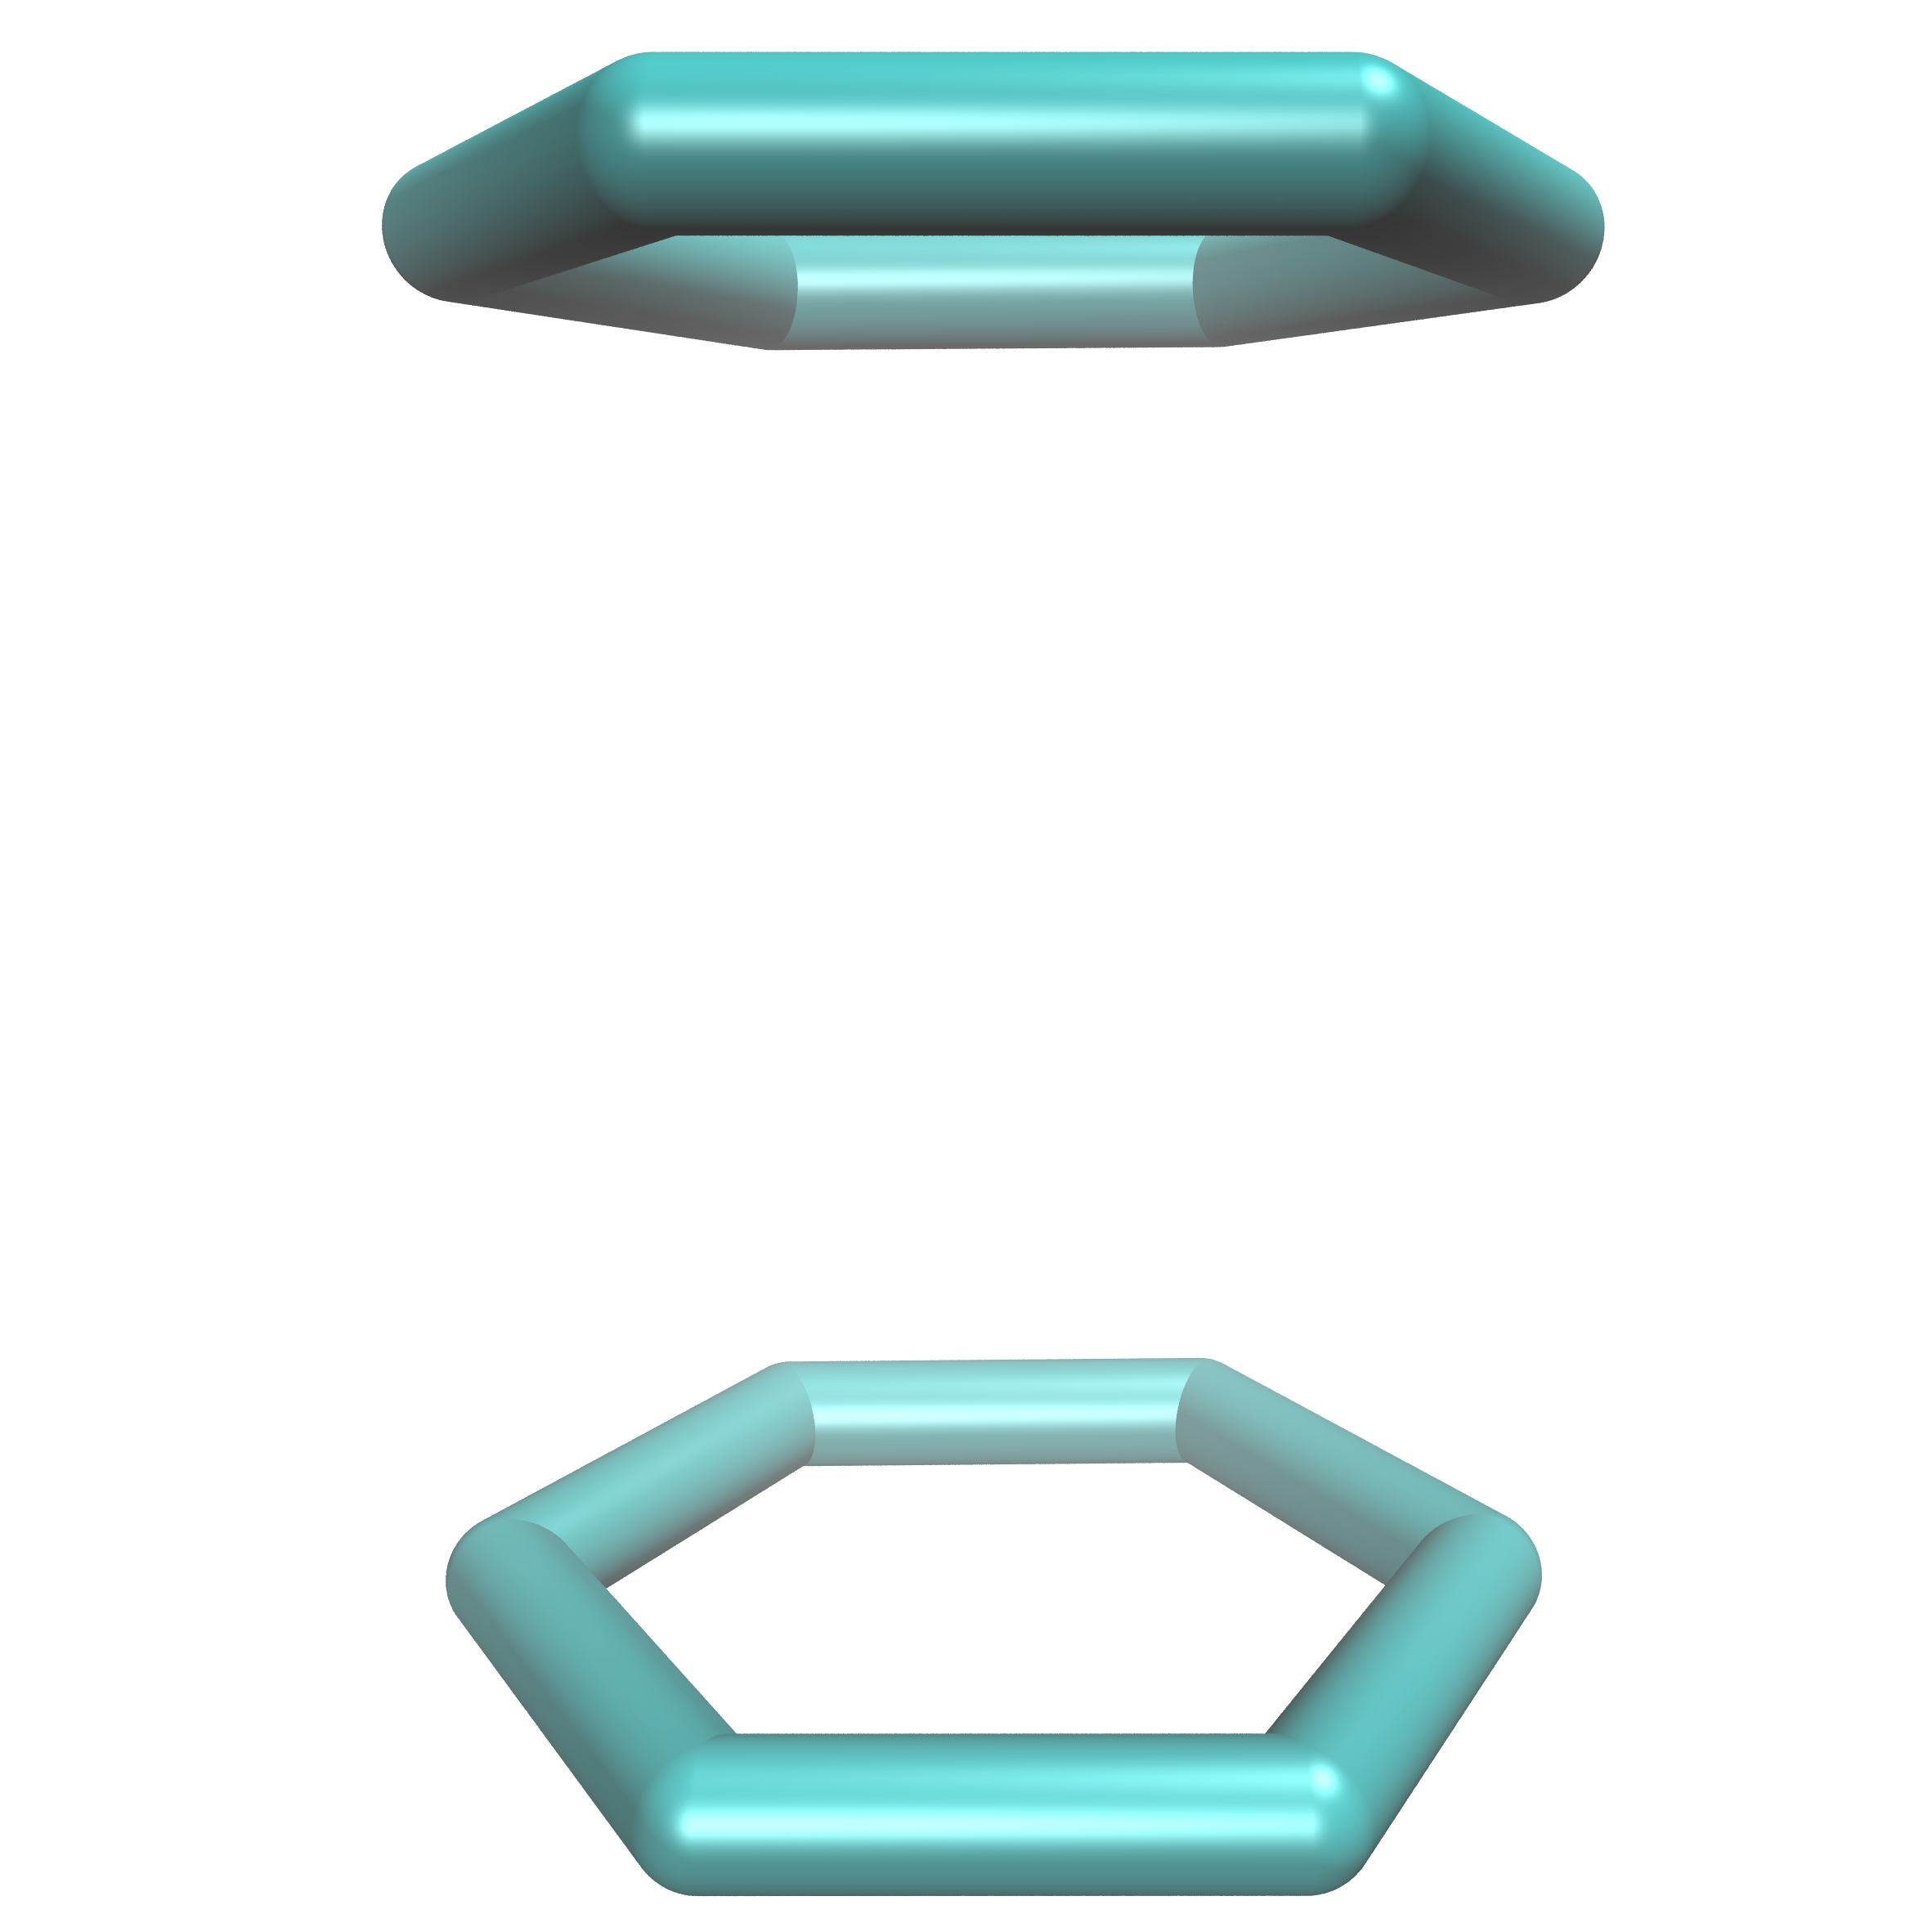
\includegraphics[width=\textwidth]{sandwiched.png}
                \caption{}\label{fig:sandwiched}
        \end{subfigure}
        \begin{subfigure}[b]{0.32\textwidth}
                \centering
                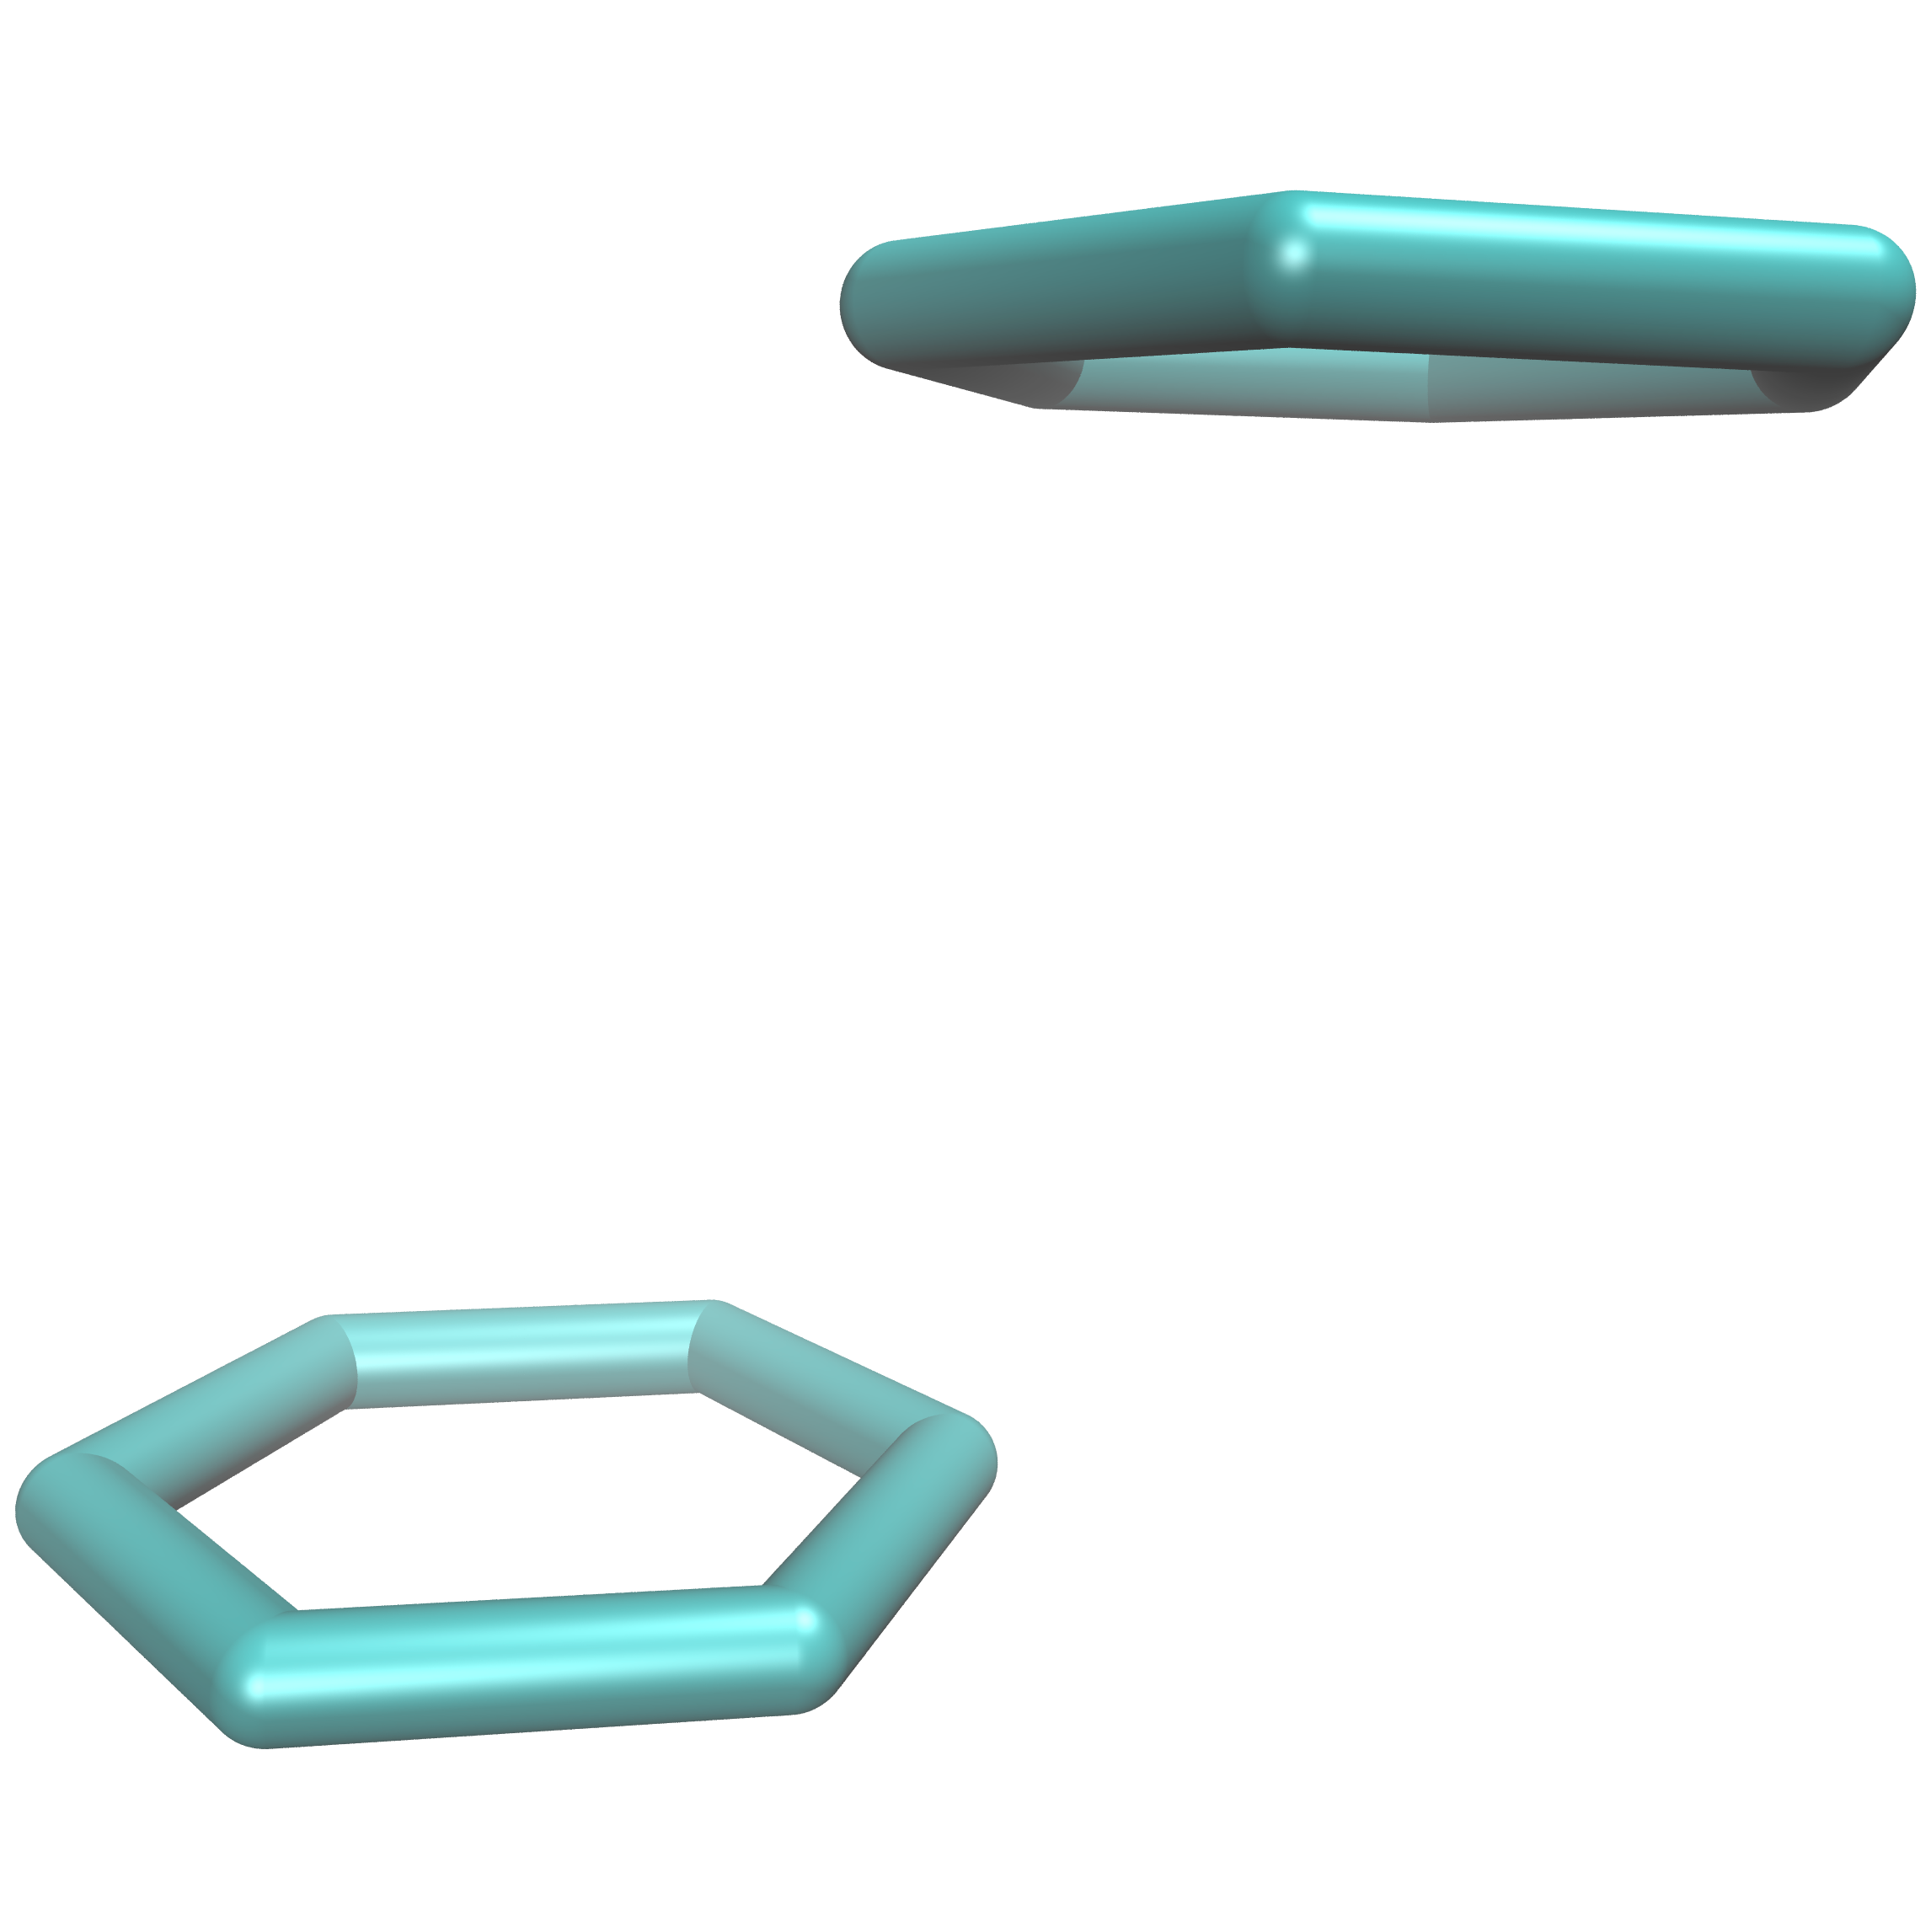
\includegraphics[width=\textwidth]{PD.png}
                \caption{}\label{fig:pd}
        \end{subfigure}
        \begin{subfigure}[b]{0.32\textwidth}
                \centering
                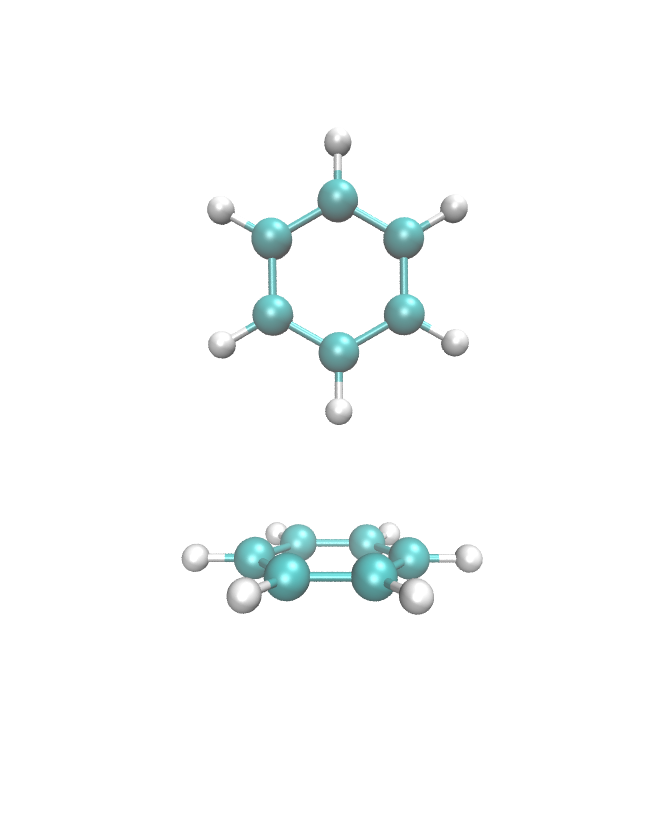
\includegraphics[width=\textwidth]{Tshaped.png}
                \caption{}\label{fig:tshaped}
        \end{subfigure}
        \vskip\baselineskip
        \begin{subfigure}[b]{0.475\textwidth}
                \centering
                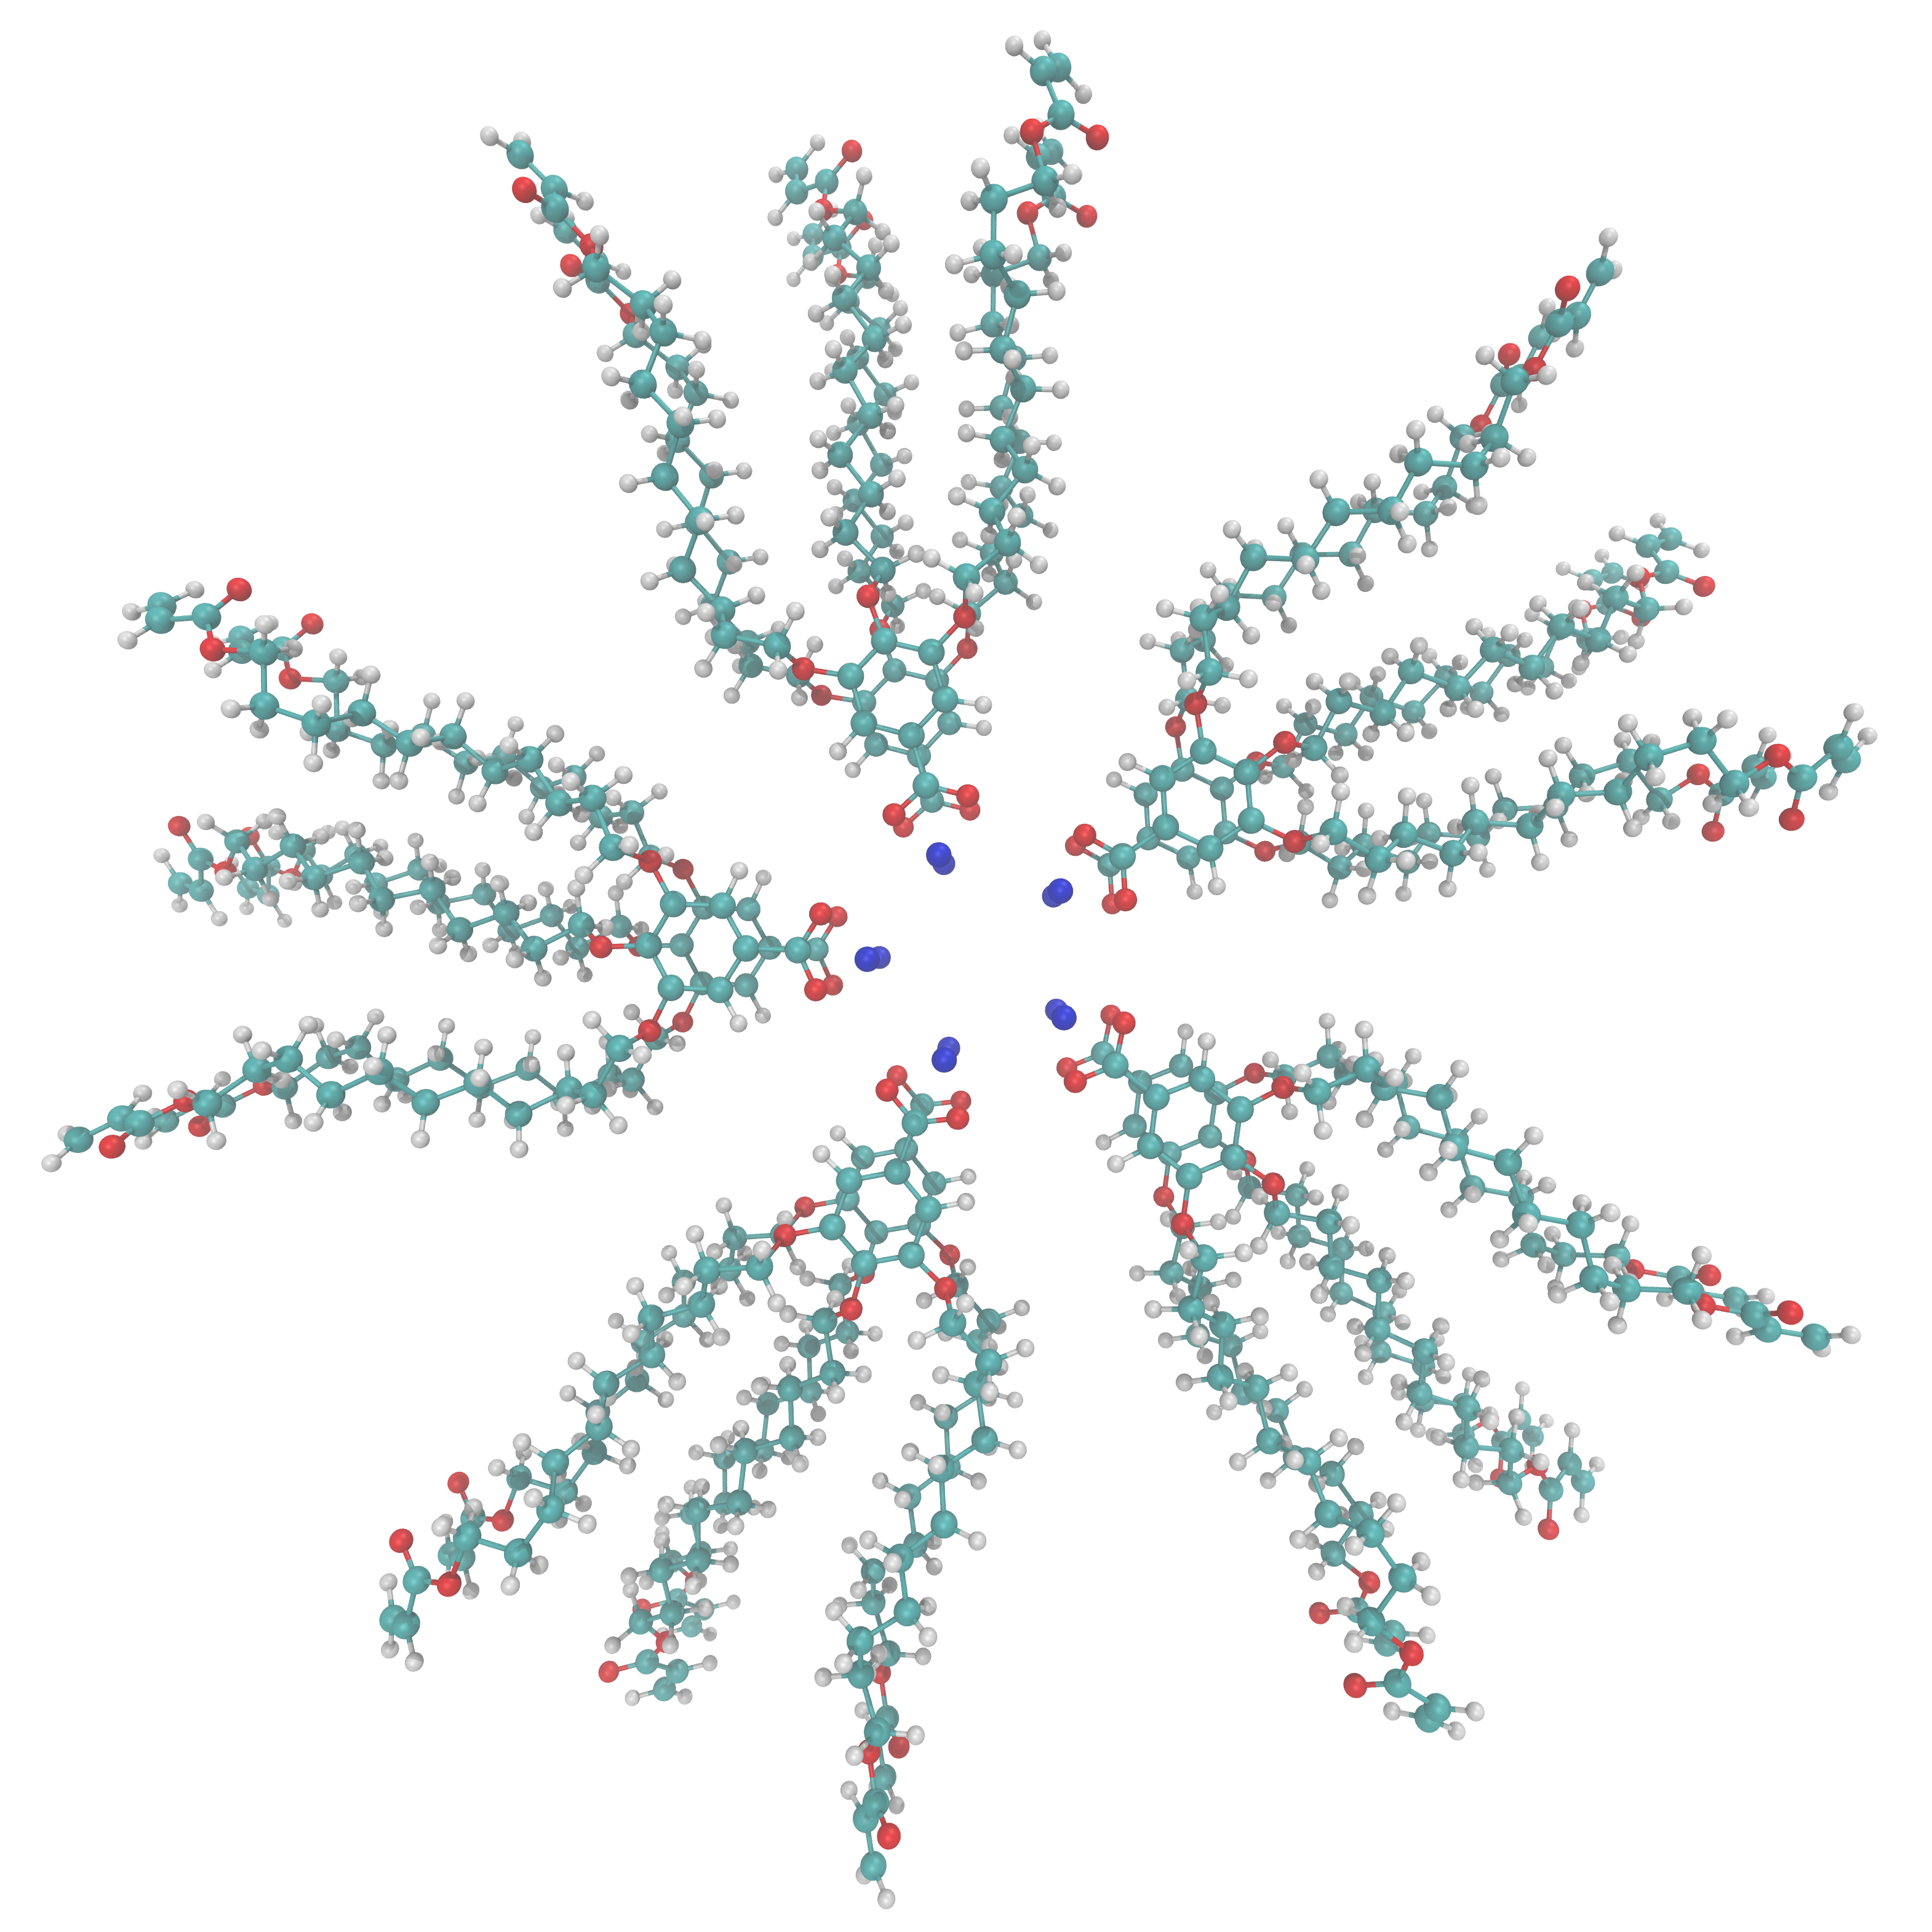
\includegraphics[width=\textwidth]{sandwichedlayers.png}
                \caption{}\label{fig:sandwichedlayers}
        \end{subfigure}
        \begin{subfigure}[b]{0.475\textwidth}
                \centering
                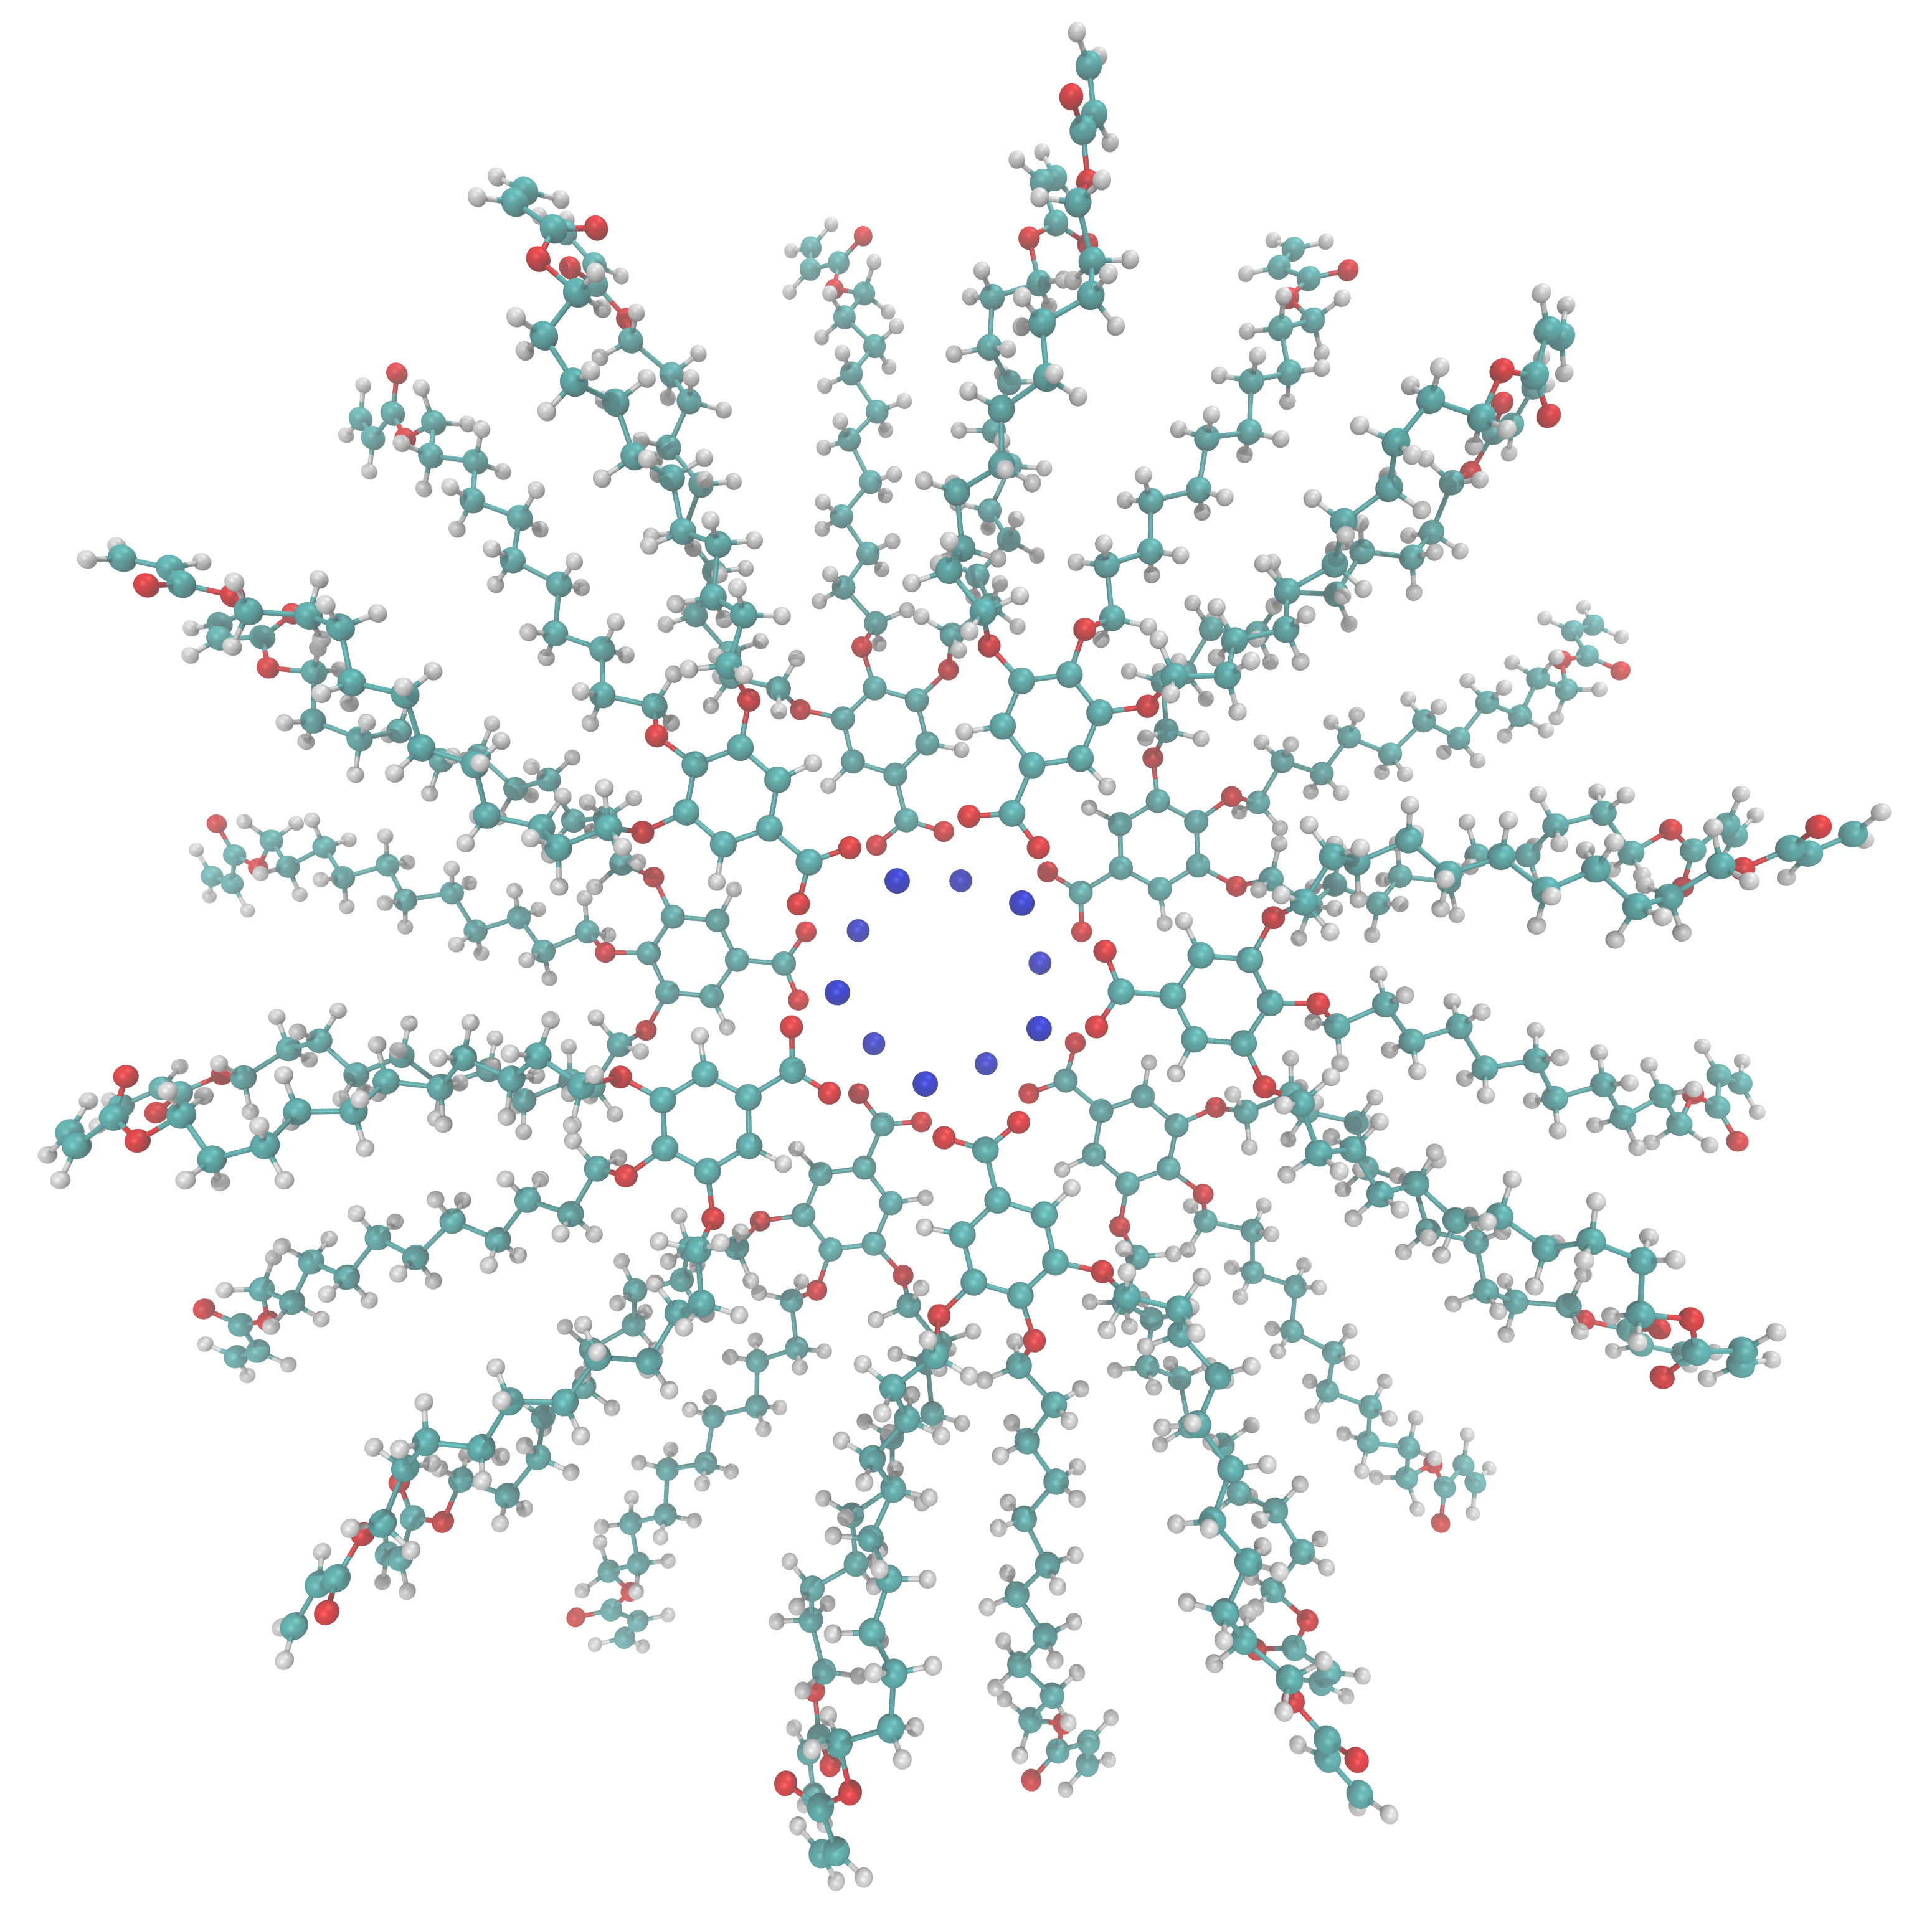
\includegraphics[width=\textwidth]{offsetlayers.png}
                \caption{}\label{fig:offsetlayers}
        \end{subfigure}
        \caption{(a) Sandwiched benzene dimers stack 3.8 \angstrom~apart. (b) Parallel-Displaced benzene dimers stack
        3.4 \angstrom~vertically and 1.6 \angstrom~horizontally apart. (c) T-shaped benzene dimers stack 5.0 \angstrom~apart.
        (d) Two monomer layers stacked in the sandwiched configuration (e) Two monomer layers stacked in the parallel-displaced
        configuration }\label{fig:stacking}
  \end{figure}

  \begin{figure}
	\centering
        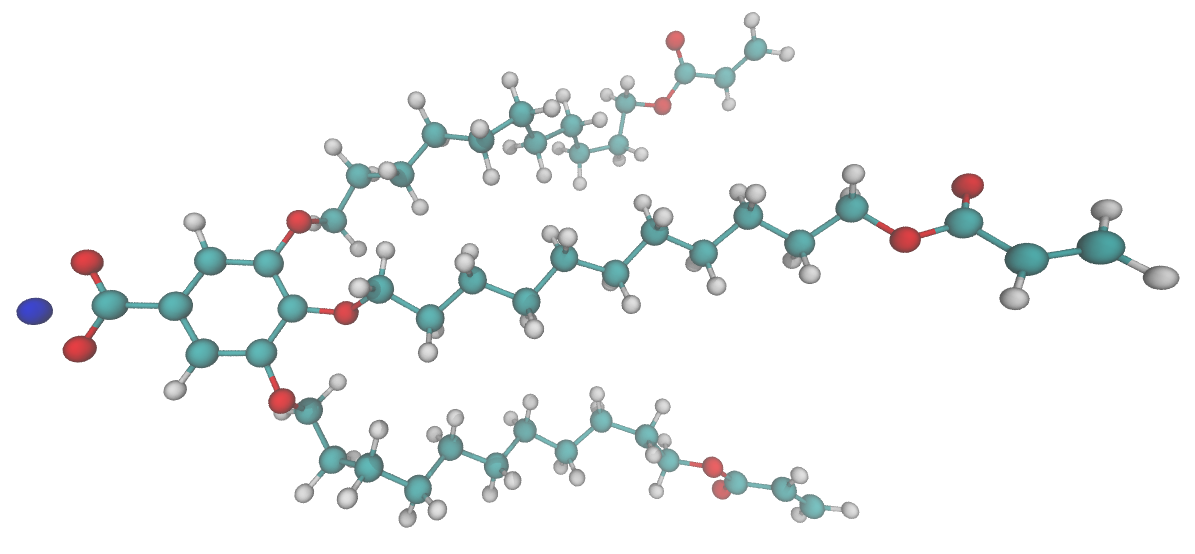
\includegraphics[width=0.9\textwidth]{monomer.png}
	\caption{Atomistic representation of the monomer Na-GA3C11. White atoms
		represent hydrogen, cyan atoms represent carbon, red atoms represent oxygen and
		the blue atom is sodium.}\label{fig:monomer}
  \end{figure}

  \begin{figure}
	\centering
        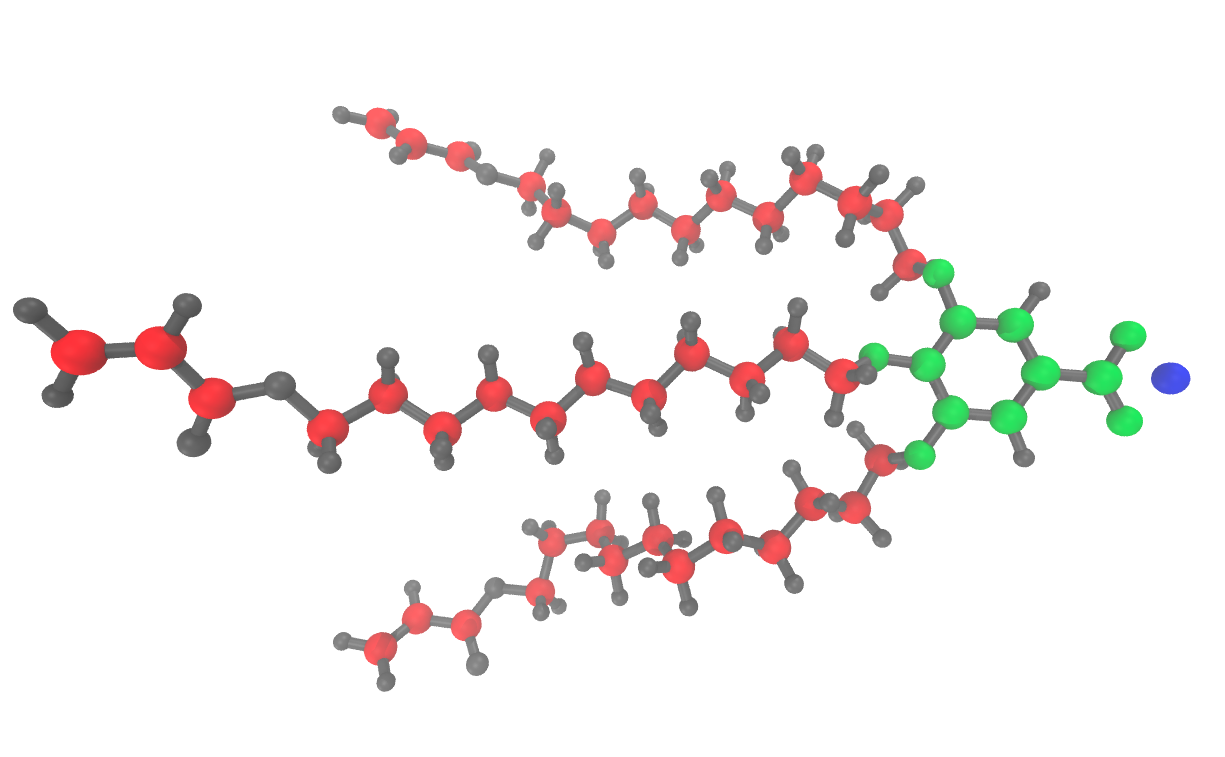
\includegraphics[width=0.9\textwidth]{monomer_color_coded.png}
	\caption{The groups used for $g(z)$ calculations. Red atoms are in the
		tails group. Green atoms are in the head group region. The blue atom is sodium. 
		}\label{fig:monomer_color_coded}
  \end{figure}

  \begin{figure}
	\centering
	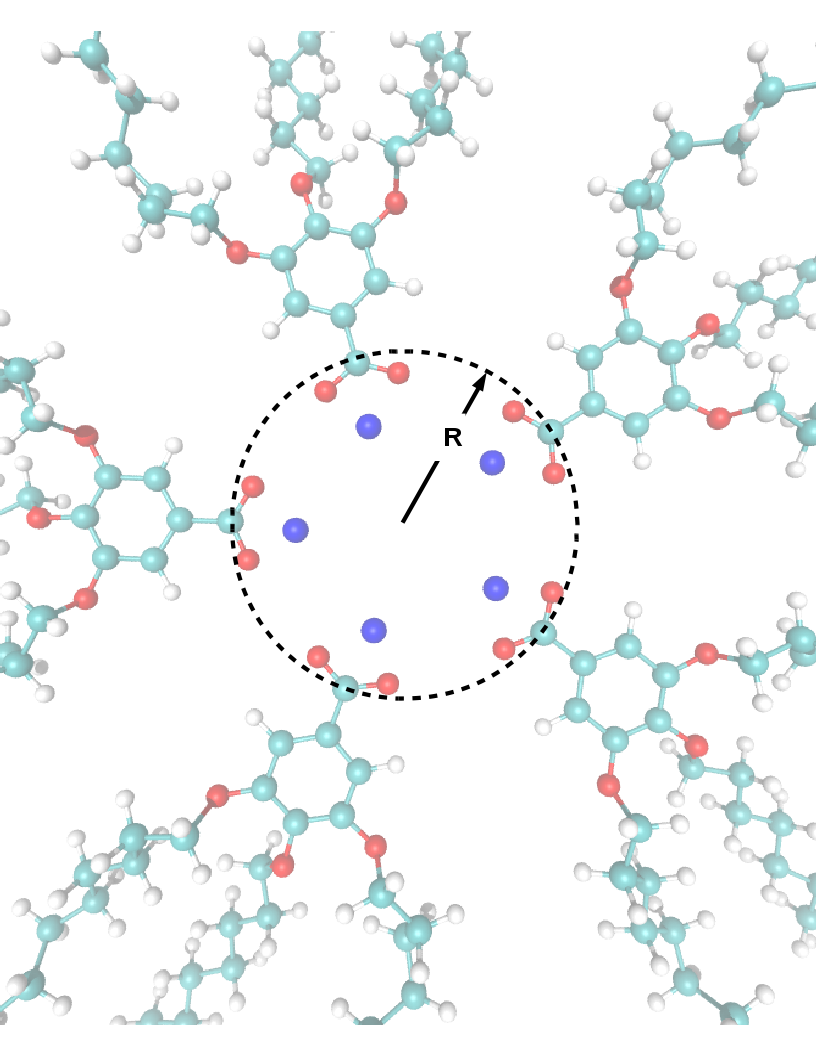
\includegraphics[width=0.8\textwidth]{pore_radius_illustration.png}
	\caption{When creating an initial configuration, the pore radius is defined based
	on the distance of the carbonyl carbon from the pore's central axis}
	\label{fig:pore_radius_illustration}
  \end{figure}

  \textbf{Calculation of pore-to-pore spacing statistics}
  
  \color{red}{This is an outline of this section and will be reworded for clarity}
  \begin{itemize}
  	\item We are interested in 5 pore-to-pore distances which should all
	be equal in a perfect hexagonal array, however only 4 distances are independent
	% can visualize this in supplemental material. Will make a lot of things more
	clear below.
	\item Each pore spacing has its own trajectory of spacing vs. time.
	Using data collected after the system is equilibrated, we calculate how long it
	takes for the data in each of the 5 trajetories to become uncorrelated using
	pymbar.timeseries.integratedAutocorrelationTime() % reference
	\item We break the full trajectories down into sub-trajectories based
	on the maximum autocorrelation time of those found in the previous step.
	\item For each bootstrap trial, we recreate an equilibrium trajectory
	by randomly sampling pore spacings from the sub-trajectories 
	\item We get an average value for each pore spacing by finding the
	mean of the bootstrapped data
	\item We calculate the overall average as the mean of all
	bootstrapped pore spacings
	\item The uncertainty for each pore spacing is calculated as
	$\dfrac{<x> - x}{4}$ where $<x>$ is the average spacing from the bootstrap
	trial and $x$ is the average value of one of the pore spacings.
	\item We report the mean of these uncertainties
  \end{itemize}

  \begingroup
	\fontsize{14pt}{12pt}\selectfont
	\textbf{Initial Configuration Dependence}
  \endgroup

  \vspace{1em}
  We addressed any major dependence on initial configuration in the main text.
  There we showed that systems are stable when made with 4, 5, 6, 7, and 8
  monomers per layer. We also showed that systems are stable when monomer head
  groups are oriented in the parallel displaced and sandwiched configurations
  (See Figure~\ref{fig:stacking}). Our model best supports a system built with 5
  monomers per layer in the sandwiched configuration. 

  There are three other parameters whose choice may influence the equilibrium
  structure: initial pore spacing, initial pore radius and initial distance
  between layers. Here we show the results of a sensitivity analysis performed
  on the three parameters. To reduce the size of the sensitivity analysis, we
  only tested systems built with 5 monomers per layer with layers stacked in 
  the parallel displaced configuration. We equilibrated all systems according
  to the dry equilibration procedure.

  %Our model is insensitive to initial configuration if monomer placement is chosen within reason. 

  \begin{enumerate}

	  \item \underline{Initial pore spacing}

	  We tested five different initial pore spacings, defined as the
	  distance between the central axis of each pore with all others. To reduce the
	  number of variables, we held the pore radius constant, at 6 \AA~and the
	  distance between layers at 3.7 \AA~since those were the values used in our
	  optimal system in the main text. If the initial pore spacing is chosen to be
	  too small, pore columns abruptly repel each other as soon as they are able to
	  overcome the restraining potential present as part of the dry equilibration
	  procedure. We avoided using systems that exhibit this behavior since the
	  behavior increases the chances of a system to become kinetically trapped in an
	  undesired metastable free energy basin.  

	  \begin{enumerate}

	  	\item 39 \AA~: We tested a pore spacing of 39 \AA~in order to have a test system
		with an intial spacing below the experimental value. As soon as the restraining
		potential switches to 56 KJ mol$^{-1}$ nm$^{-2}$, the columns are able to
		separate resulting in a large jump in pore spacing (Figure~\ref{fig:p2p_39}). 

		\item 41 \AA~: We chose to test a pore spacing of 41 \AA~since
		it closely matches the experimental pore spacing. Again, we observe abrupt
		repulsion of columns once the restraining potential is switched to 56 KJ
		mol$^{-1}$ nm$^{-2}$ (Figure~\ref{fig:p2p_41}).

		\item 45 \AA~: A pore spacing of 45 \AA~is about 10 \% larger than the
		experimental value. We observe relatively stable pore spacing during the
		restrained portion of the dry equilibration procedure
		(Figure~\ref{fig:p2p_45}). We chose to use this value for all our simulations
		in the main text. 

		\item 50 \AA~: We tested a pore spacing of 50 \AA, about 20 \% larger than the
		experimental value. Once the restraining potential reaches 56 KJ mol$^{-1}$
		nm$^{-2}$, the pore spacing begins to decrease linearly (Figure~\ref{fig:p2p_50}).

		\item 55 \AA~: We tested a pore spacing of 55 \AA~ which is at
		a distance where monomers in each pore no longer intersect adjacent pores. Once
		the restraining potential reaches 56 KJ mol$^{-1}$ nm$^{-2}$, the pore spacing
		changes erratically until it begins to settle when the force constants are
		below 3 KJ mol$^{-1}$ nm$^{-2}$ (Figure~\ref{fig:p2p_55}). We reccomend
		avoiding a system such as this where vacuum gaps between pore columns are
		introduced unnecessarily.  The system equilibrates to a pore spacing of 4.27
		$\pm$ 0.06 nm. 

	  \end{enumerate} 

	  %BJC: Could put vertical lines to indicate where position restraint values are reduced
  	  \begin{figure}[htp]
		\centering
		\begin{subfigure}{0.3\textwidth}
			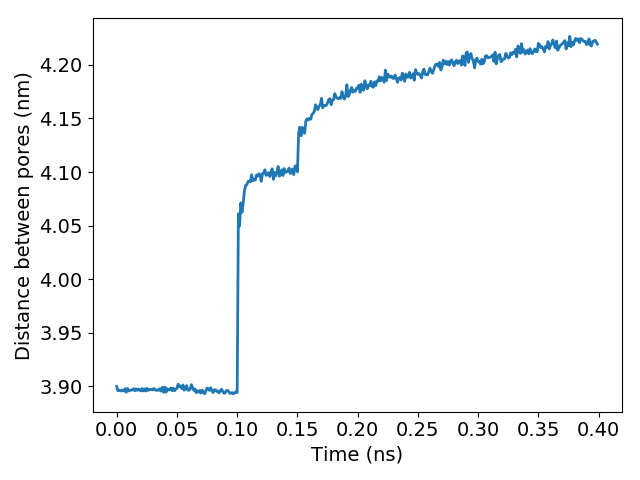
\includegraphics[width=\textwidth]{p2p_39.png}\quad
			\vspace{-1.25em}
			\caption{39 \AA~initial pore spacing}~\label{fig:p2p_39}
		\end{subfigure}
		\begin{subfigure}{0.3\textwidth}
			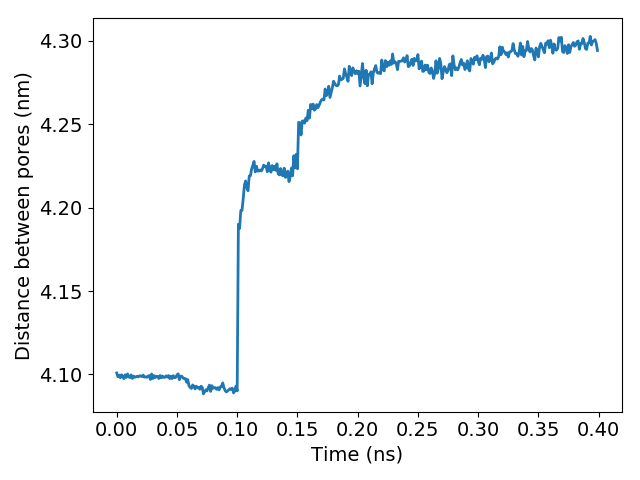
\includegraphics[width=\textwidth]{p2p_41.png}\quad
			\vspace{-1.25em}
			\caption{41 \AA~initial pore spacing}~\label{fig:p2p_41}
		\end{subfigure}
		\begin{subfigure}{0.3\textwidth}
			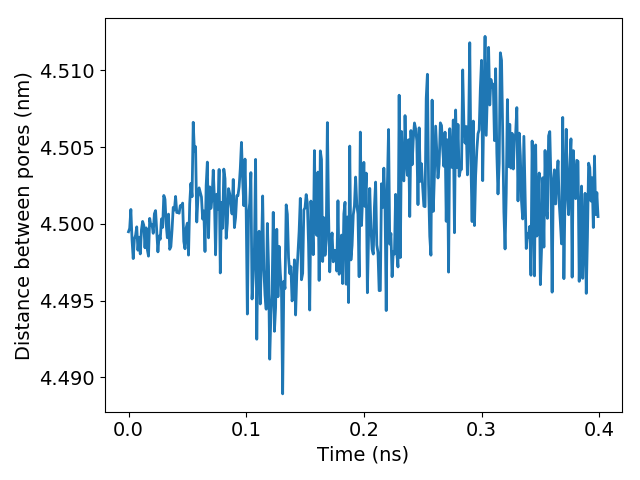
\includegraphics[width=\textwidth]{p2p_45.png}
			\vspace{-1.25em}
			\caption{45 \AA~initial pore spacing}~\label{fig:p2p_45}
		\end{subfigure}
		\begin{subfigure}{0.3\textwidth}
			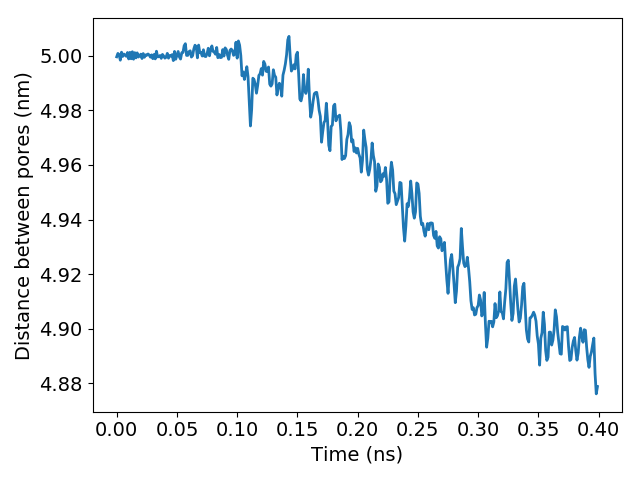
\includegraphics[width=\textwidth]{p2p_50.png}\quad	
			\vspace{-1.25em}
			\caption{50 \AA~initial pore spacing}~\label{fig:p2p_50}
		\end{subfigure}
		\begin{subfigure}{0.3\textwidth}
			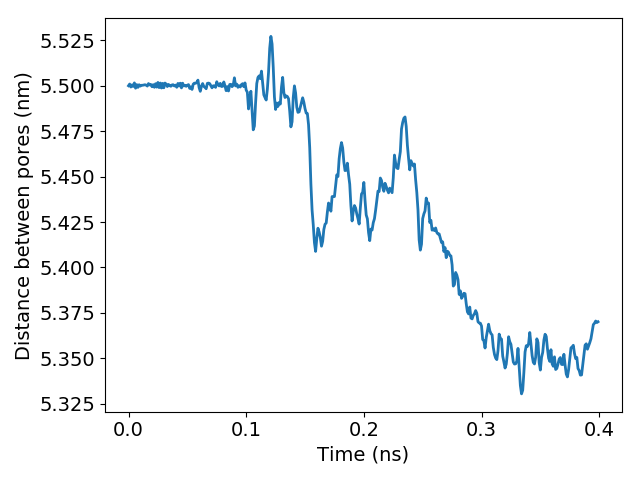
\includegraphics[width=\textwidth]{p2p_55.png}
			\vspace{-1.25em}
			\caption{55 \AA~initial pore spacing}~\label{fig:p2p_55}
		\end{subfigure}

		\caption{The pore spacing during the restrained portion of the
			dry equilibration procedure is shown. Every 50 ps (0.05 ns) position restraints
			are reduced according to the sequence: 1000000, 3162, 56, 8, 3, 2, 1, 0 KJ
			mol$^{-1}$ nm$^{-2}$. When the initial pore spacing is chosen below the
			experimental value (a) or at the experimental value (b), there is an abrupt
			change in pore spacing when the position restraints are reduced to 56 KJ
			mol$^{-1}$ nm$^{-2}$. When pores are started 45 \AA~apart (c) the pore spacing
			remains relatively stable. When pores are spaced 50 \AA~apart (d), the pore
			spacing decreases nearly linearly once the restraints are reduced to 56 KJ
			mol$^{-1}$ nm$^{-2}$. When pores are spaced 55 \AA~apart (e), so that monomers
			do not intersect with adjacent pores, and position restraints are reduced to 56
			KJ mol$^{-1}$ nm$^{-2}$, the pore spacing changes erratically before stabilizing
			when force constants are reduced below 3 KJ mol$^{-1}$ nm$^{-2}$.} 
		\label{fig:p2p}
	  \end{figure}

	  \item \underline{Initial pore radius}

	  We tested 3 different pore radii, defined as shown in
	  Figure~\ref{fig:pore_radius_illustration}. For each system, we held the initial
	  pore spacing constant at 45 \AA~ and the distance between layers constant at
	  3.7 \AA. Equilibrated values of pore radii are presented in
	  Table~\ref{table:radii}. The pore radius in each simulation frame is calculated as the
	  average distance of all carbonyl carbons (See
	  Figure~\ref{fig:pore_radius_illustration}) from their associated pore center.
	  Statistics for the pore radii reported were generated from the timeseries
	  representing the average pore radius at each frame.  We detected equilibration 
	  using \texttt{pymbar.timeseries.detectEquilibration}. We calculated the average
	  and standard deviation of pore radii using only data points collected after
	  equilibration was detected.

	  \begin{enumerate}

		\item 2.5 \AA~: The smallest pore radius that we can achieve before energy 
		minimization becomes problematic is 2.5 \AA.

		\item 5 \AA~: 

		\item 8 \AA~: The largest pore radius that can achieve before energy minimization
		becomes problematic is 8 \AA.
	  \end{enumerate}

	  \begin{table}[h]
	  \centering
	  \begin{tabular}{cc}
	  \toprule
	  Initial Pore Radius & Equilibrated Pore Radius \\
	  \midrule
	  % BJC: to be updated once simulations are run out long enough
	  2.5 \AA & $0.394 \pm 0.002$ \AA \\
	  5 \AA   & $0.423 \pm 0.002$ \AA \\ % final result
	  8 \AA   & $0.721 \pm 0.002$ \AA \\
	  \bottomrule
	  \end{tabular}
	  \caption{Caption of the future!}~\label{table:radii}
	  \end{table}

	  \item Initial distance between layers

	  We tested 3 different initial layer spacings, defined as the distance
	  between the planes of aromatic rings in each layer. Systems built with layers
	  stacked 3.7 \AA~and 5 \AA~apart are discussed extensively in the main text. We
	  will focus the discussion here on systems built with layers stacked 10~\AA
	  apart.

	  Figure~\ref{fig:dbwl_10} shows the structure of an assembly built
	  with an initial layer spacing of 10 \AA~immediately after the restrained
	  portion of the equilibration procedure. Since we used position restraints, the
	  simulations were run in the NVT ensemble. When layer spacing is large, such as
	  this situation, there is a significant amount of vacuum space which the monomer
	  attempts to fill. Even if turning pressure control on allows the system to
	  recover the geometry of the hexagonal phase, we would likely need much longer
	  equilibration times, and it will almost certainly get trapped in a metastable
	  configuration that bears no resemblence to the experimental profile. 
 
	  \begin{figure}
		\centering
		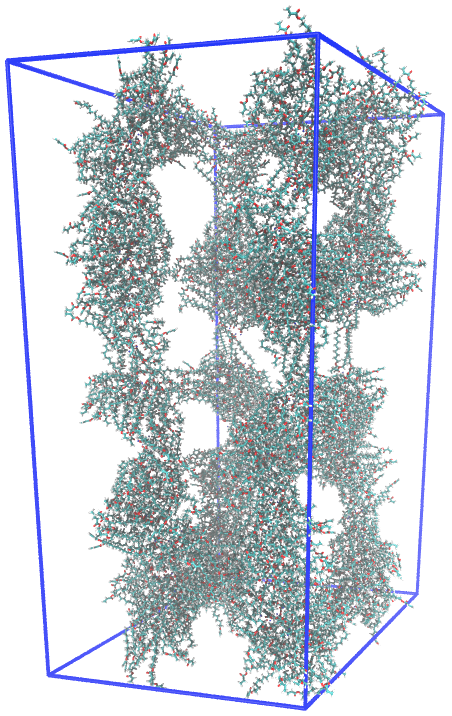
\includegraphics[width=0.5\textwidth]{dbwl_10.png}
		\caption{When layers are initially stacked 10 \AA~apart and the system
                is equilibrated using the dry equlibration procedure, large vacuum gaps
		form as the monomers attempt to fill space.}\label{fig:dbwl_10} 
	  \end{figure}

  \end{enumerate}

  \begin{figure}
	\centering
        \begin{subfigure}{0.40\textwidth}
                \centering
                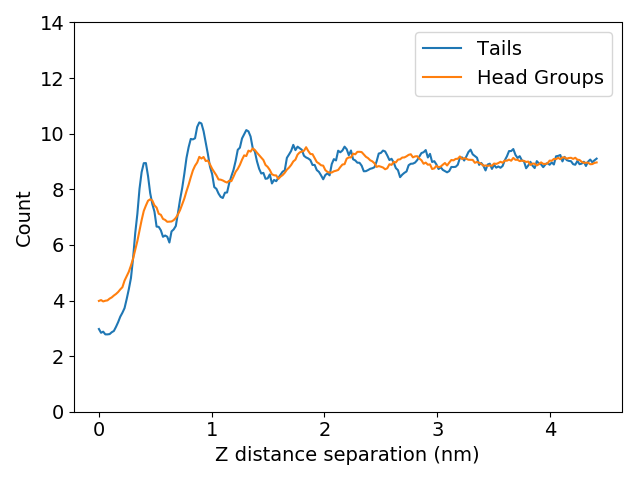
\includegraphics[width=\textwidth]{zdf_layered_4.png}
                \caption{4 mon/layer, Sandwiched}\label{fig:zdf_layered_4}
        \end{subfigure}
        \begin{subfigure}{0.40\textwidth}
                \centering
                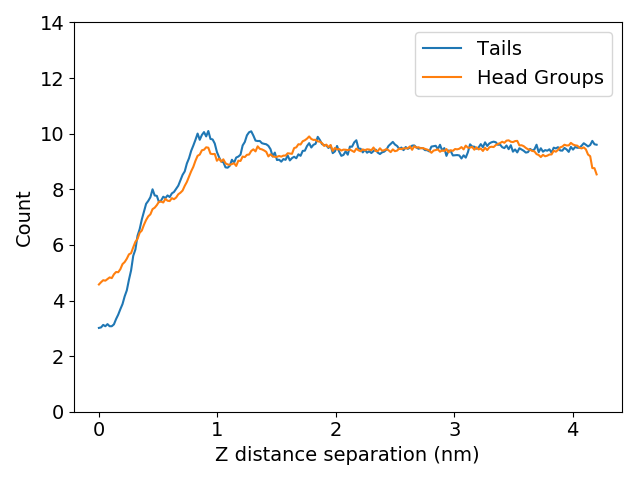
\includegraphics[width=\textwidth]{zdf_offset_4.png}
                \caption{4 mon/layer, Parallel Displaced}\label{fig:zdf_layered_4}
        \end{subfigure}
	\begin{subfigure}{0.40\textwidth}
                \centering
                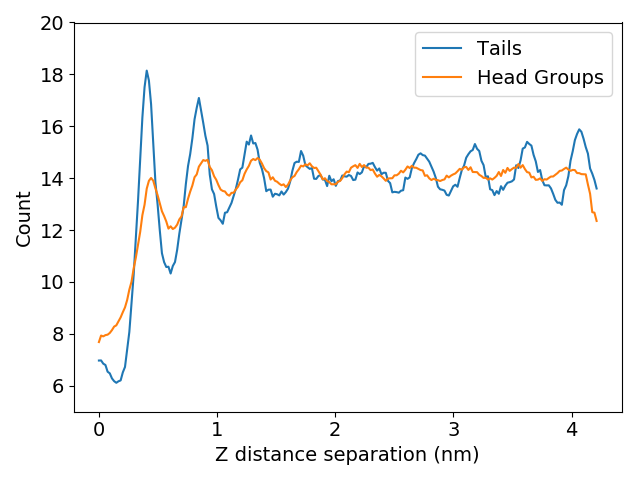
\includegraphics[width=\textwidth]{zdf_layered_6.png}
                \caption{6 mon/layer, Sandwiched}\label{fig:zdf_layered_6}
        \end{subfigure}
        \begin{subfigure}{0.40\textwidth}
                \centering
                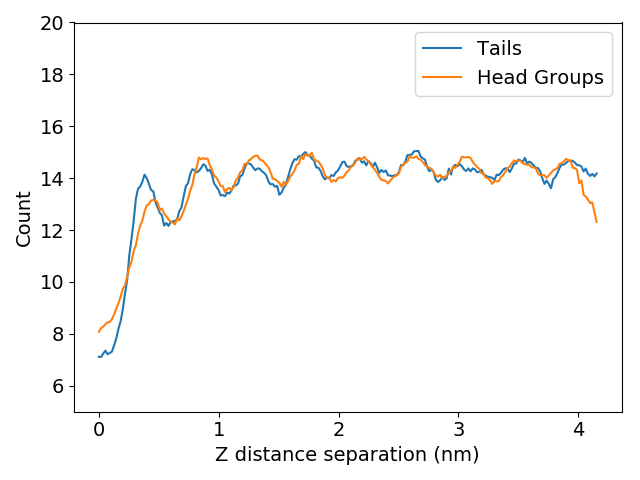
\includegraphics[width=\textwidth]{zdf_offset_6.png}
                \caption{6 mon/layer, Parallel Displaced}\label{fig:zdf_layered_6}
        \end{subfigure}
        \begin{subfigure}{0.40\textwidth}
                \centering
                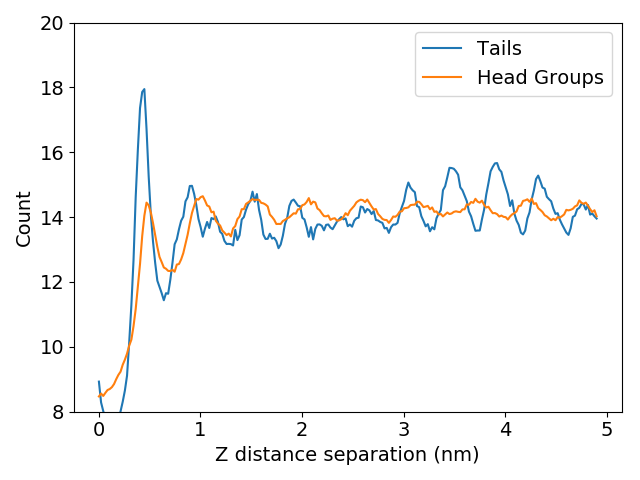
\includegraphics[width=\textwidth]{zdf_layered_7.png}
                \caption{7 mon/layer, Sandwiched}\label{fig:zdf_layered_7}
        \end{subfigure}
        \begin{subfigure}{0.40\textwidth}
                \centering
                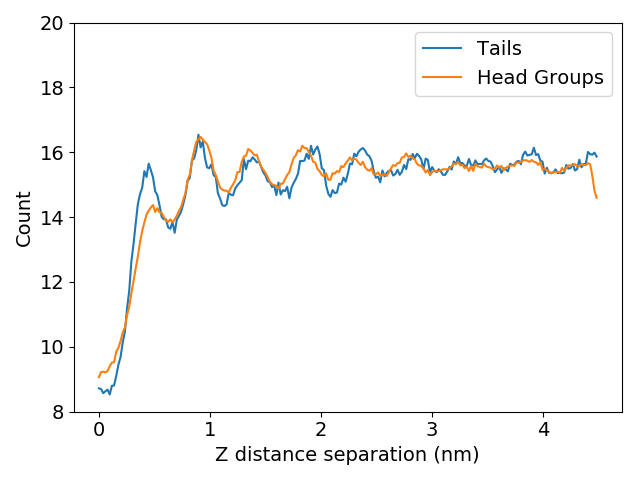
\includegraphics[width=\textwidth]{zdf_offset_7.png}
                \caption{7 mon/layer, Parallel Displaced}\label{fig:zdf_layered_7}
        \end{subfigure}
	\begin{subfigure}{0.40\textwidth}
                \centering
                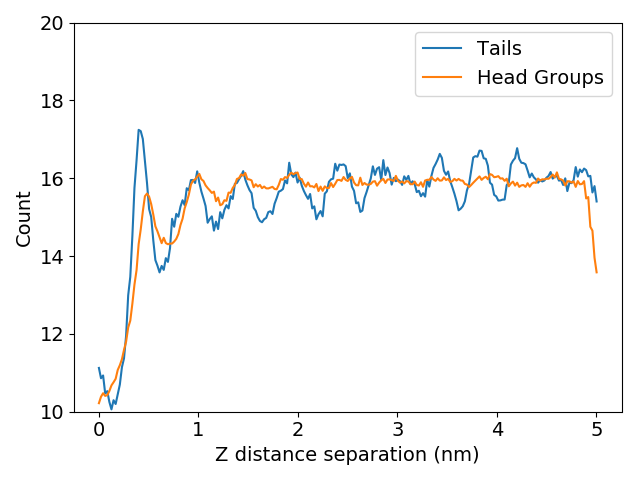
\includegraphics[width=\textwidth]{zdf_layered_8.png}
                \caption{8 mon/layer, Sandwiched}\label{fig:zdf_layered_8}
        \end{subfigure}
        \begin{subfigure}{0.40\textwidth}
                \centering
                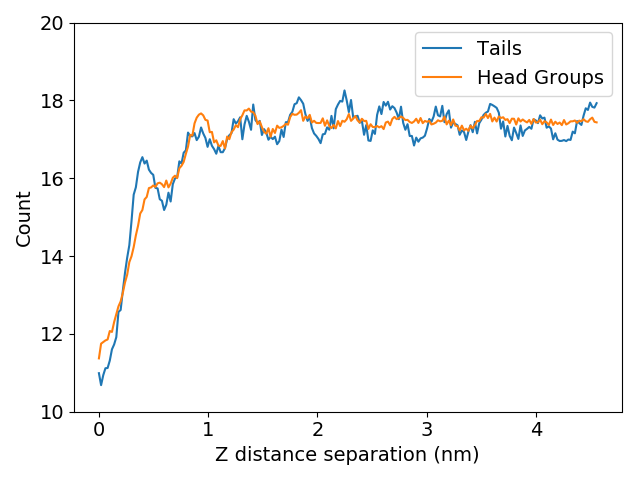
\includegraphics[width=\textwidth]{zdf_offset_8.png}
                \caption{8 mon/layer, Parallel Displaced}\label{fig:zdf_layered_8}
        \end{subfigure}
	\caption{$g(z)$ for all other configurations built with layers stacked 3.7 \AA~apart}\label{fig:zdf}
  \end{figure}

  \begin{figure}
	\centering
        \begin{subfigure}{0.40\textwidth}
                \centering
                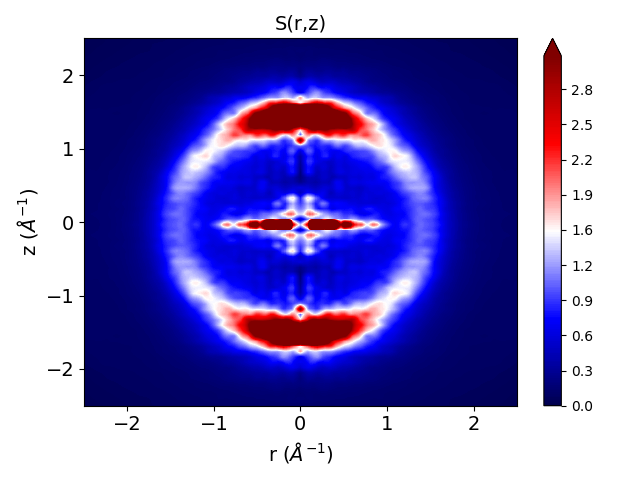
\includegraphics[width=\textwidth]{rzplot_layered_4.png}
                \caption{4 mon/layer, Sandwiched}\label{fig:rzplot_layered_4}
        \end{subfigure}
        \begin{subfigure}{0.40\textwidth}
                \centering
                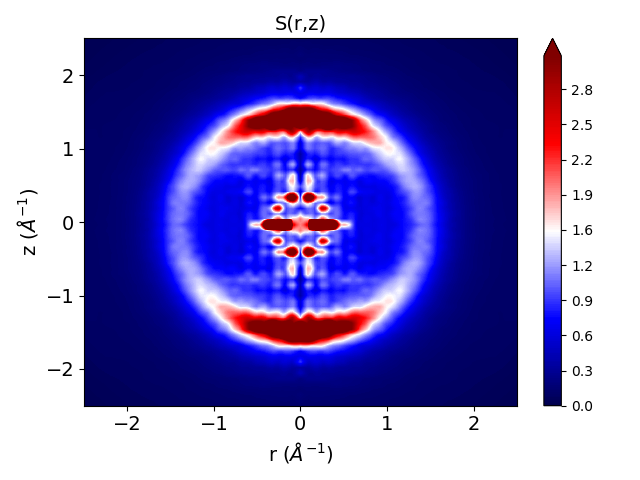
\includegraphics[width=\textwidth]{rzplot_offset_4.png}
                \caption{4 mon/layer, Parallel Displaced}\label{fig:rzplot_offset_4}
        \end{subfigure}
        \begin{subfigure}{0.40\textwidth}
                \centering
                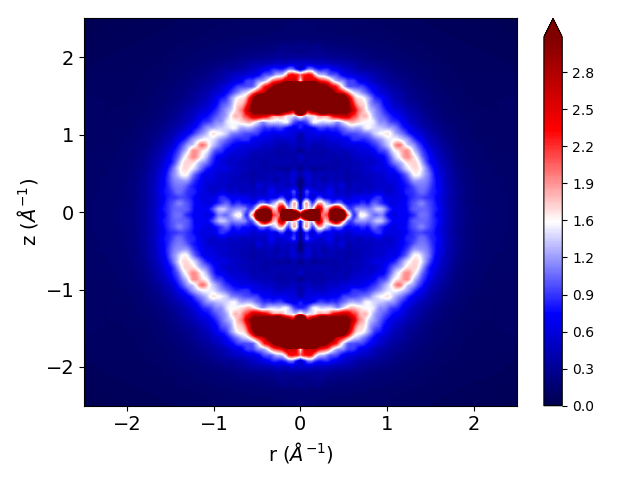
\includegraphics[width=\textwidth]{rzplot_layered_6.png}
                \caption{6 mon/layer, Sandwiched}\label{fig:rzplot_layered_6}
        \end{subfigure}
        \begin{subfigure}{0.40\textwidth}
                \centering
                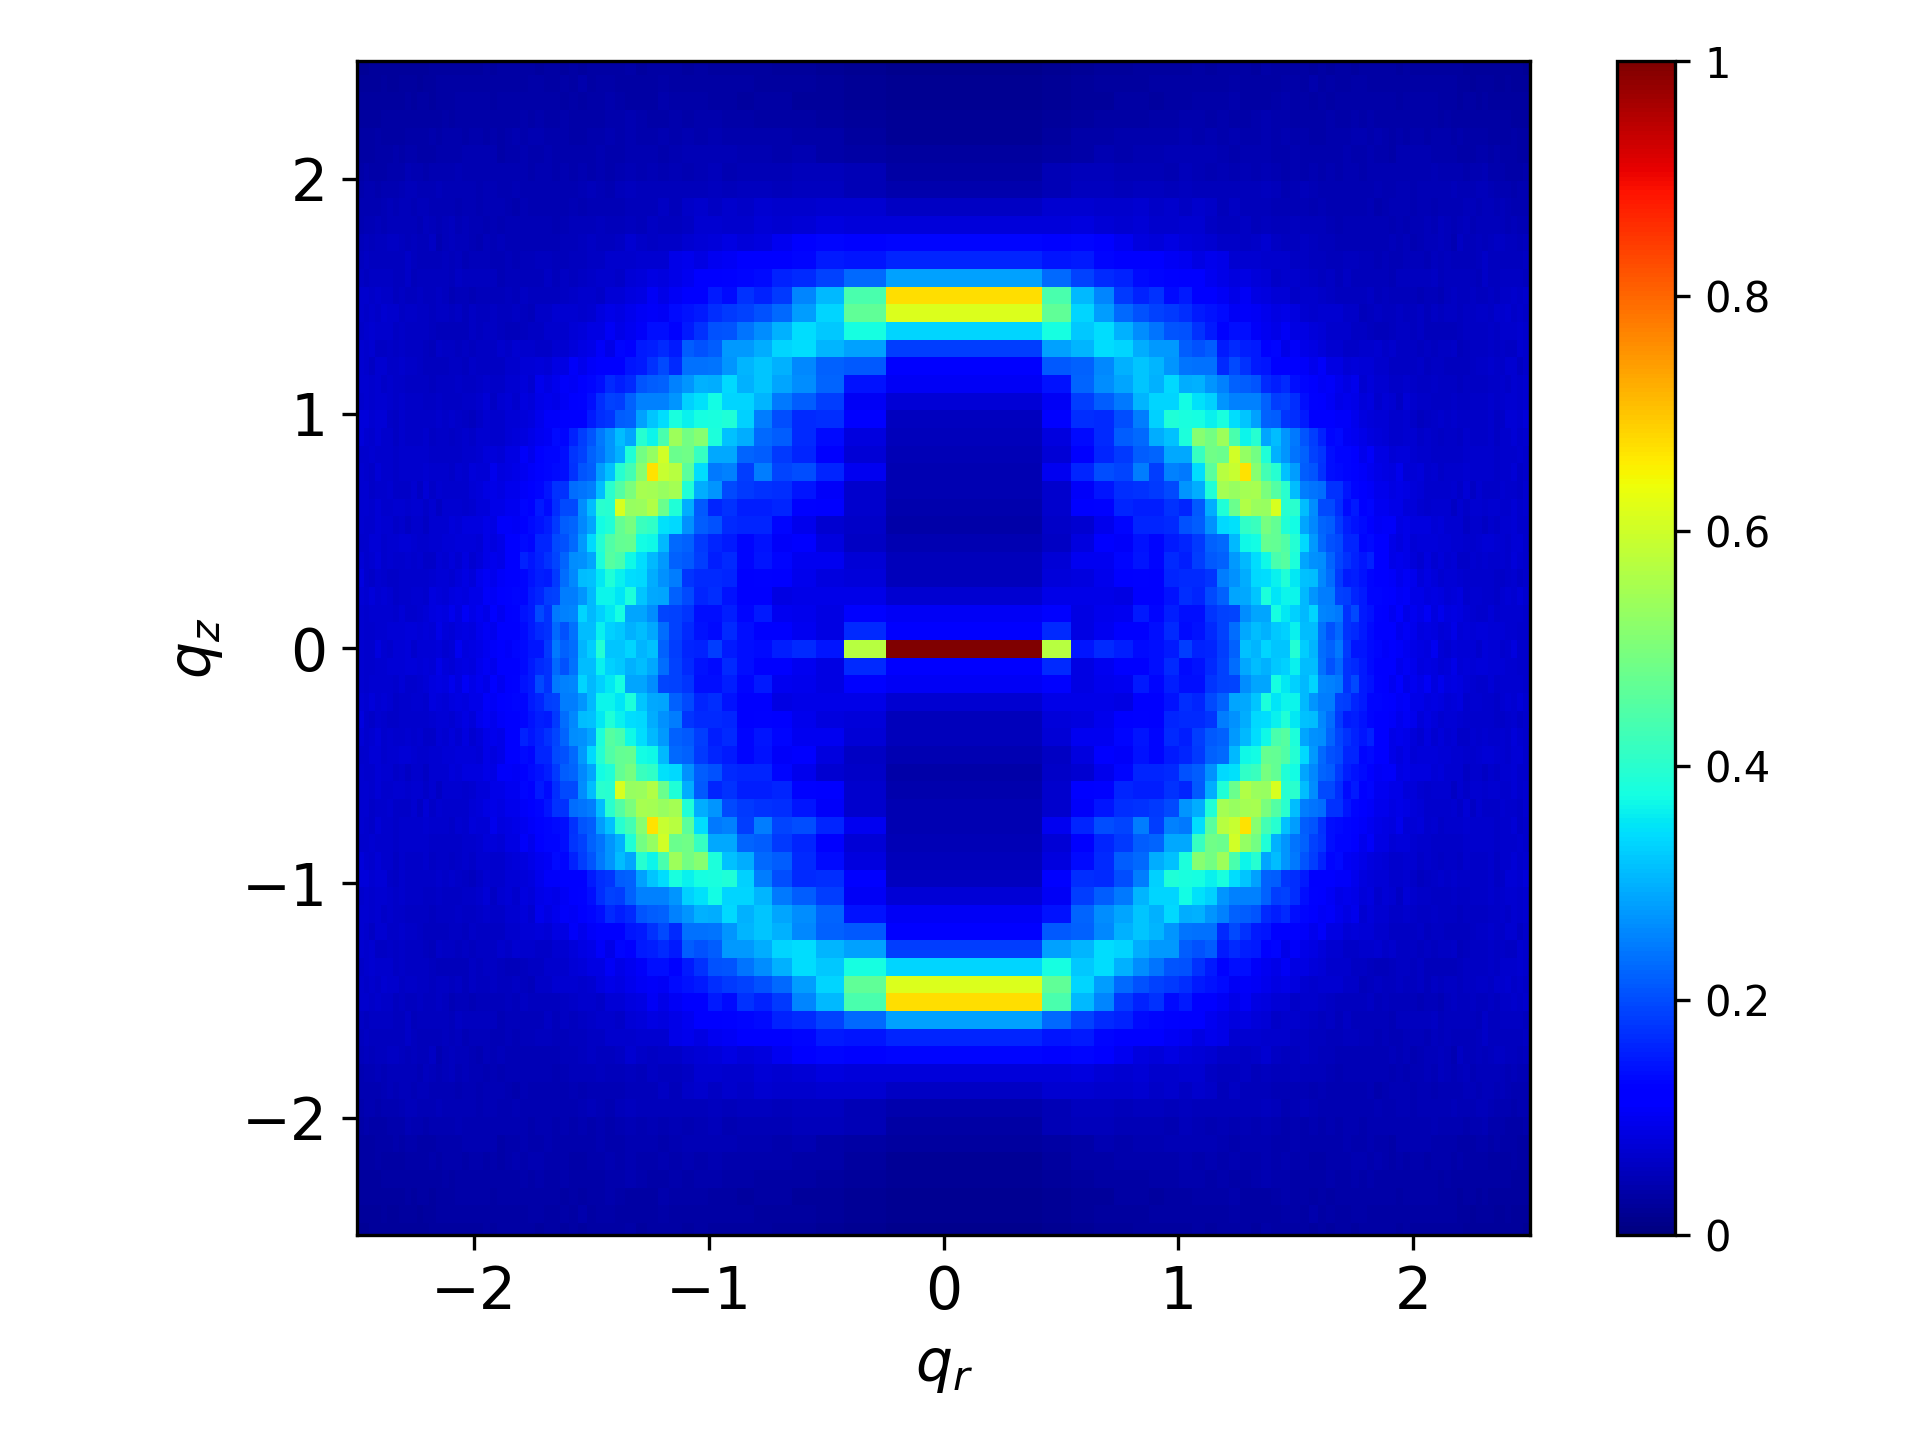
\includegraphics[width=\textwidth]{rzplot_offset_6.png}
                \caption{6 mon/layer, Parallel Displaced}\label{fig:rzplot_offset_6}
        \end{subfigure}
        \begin{subfigure}{0.40\textwidth}
                \centering
                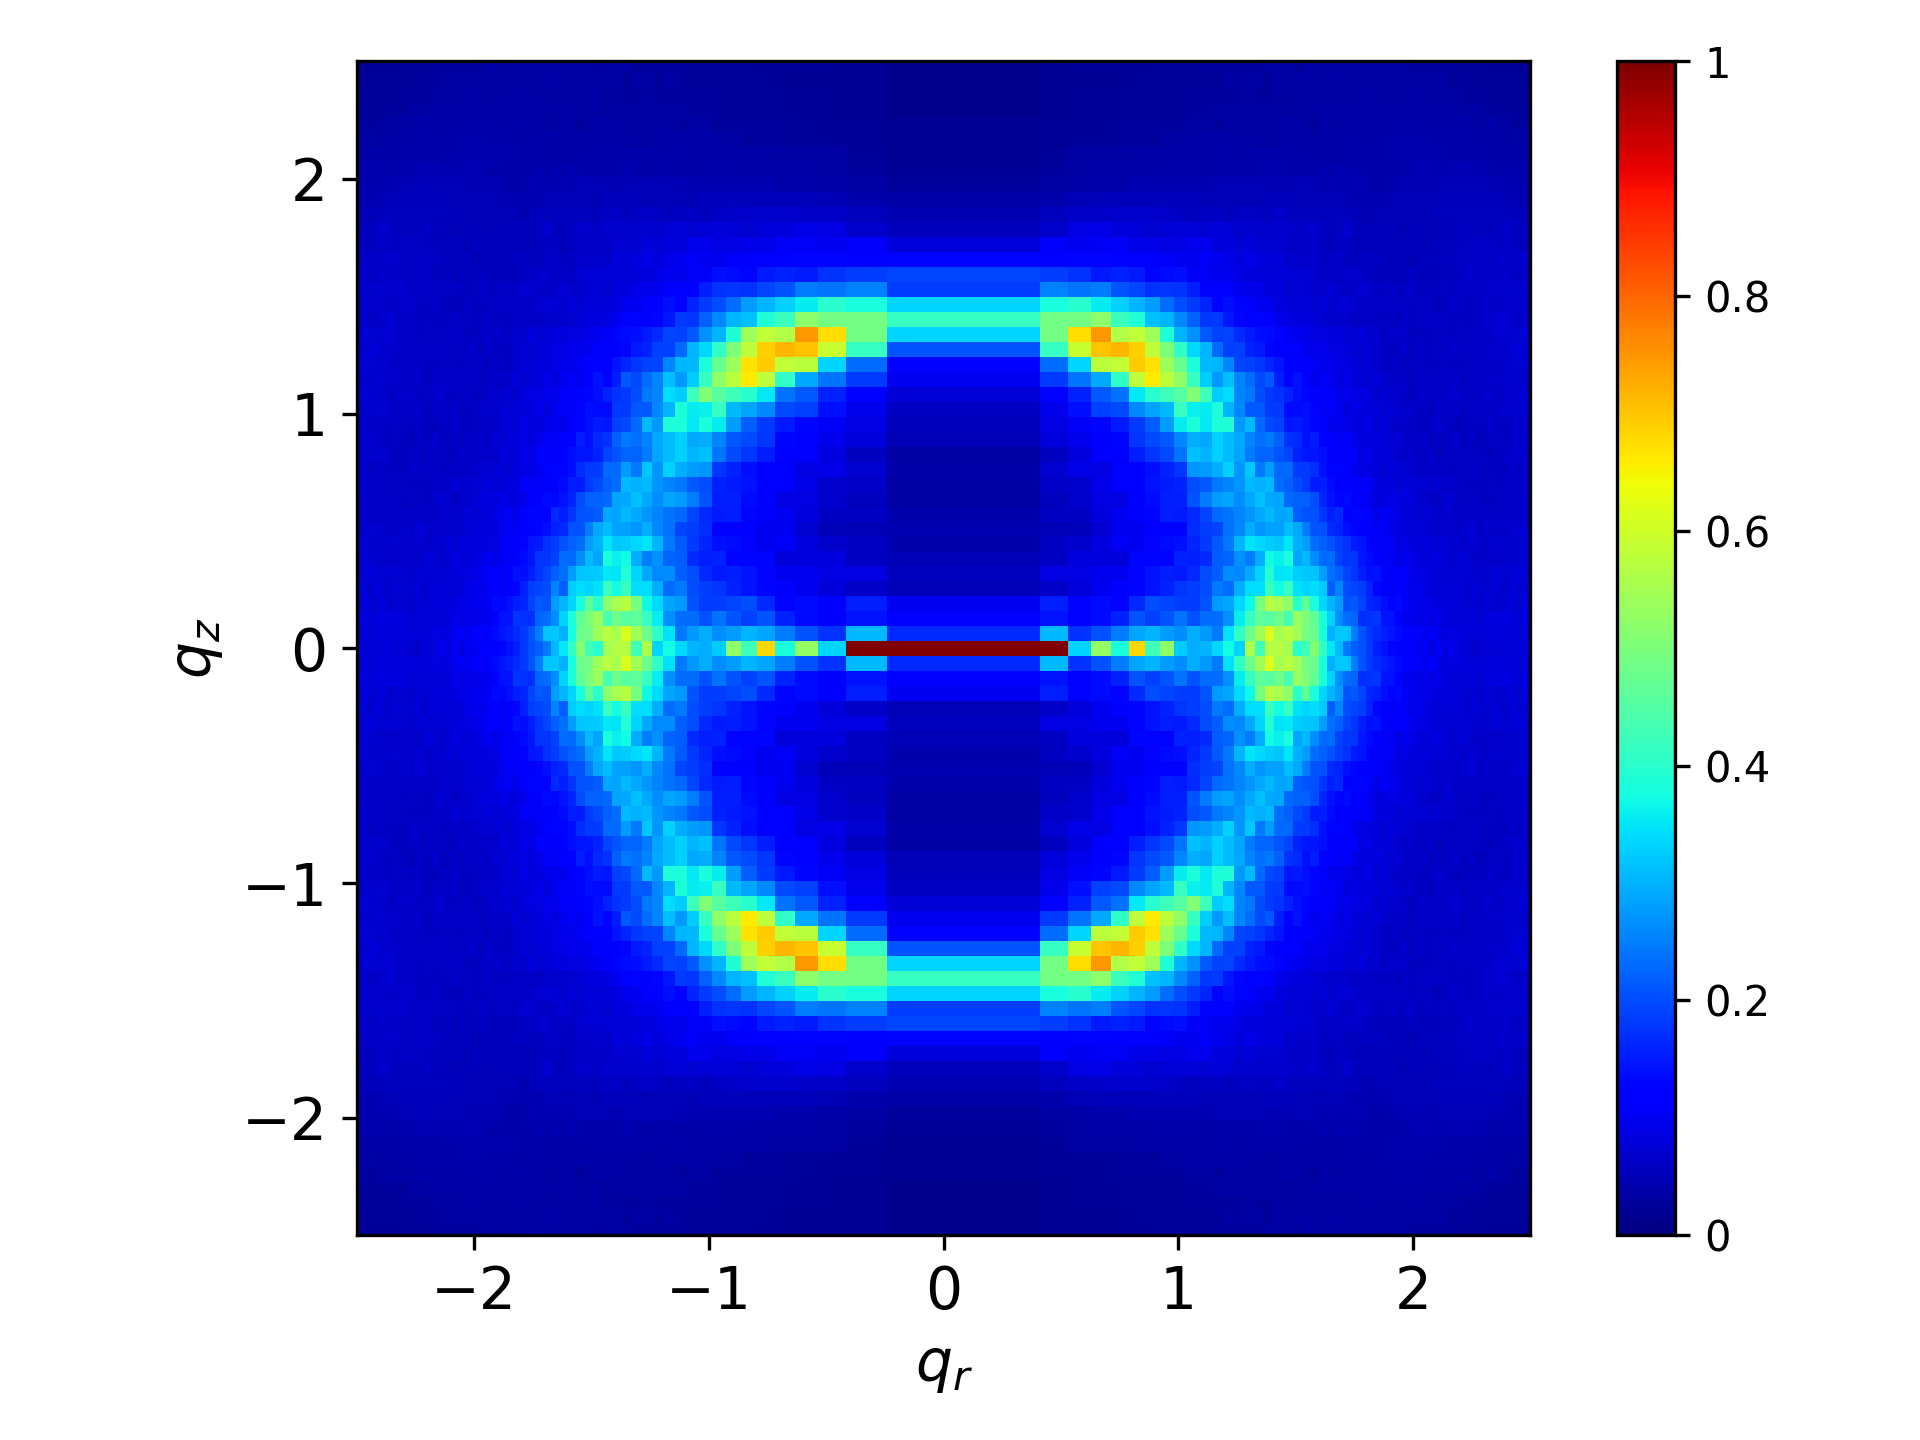
\includegraphics[width=\textwidth]{rzplot_layered_7.png}
                \caption{7 mon/layer, Sandwiched}\label{fig:rzplot_layered_7}
        \end{subfigure}
        \begin{subfigure}{0.40\textwidth}
                \centering
                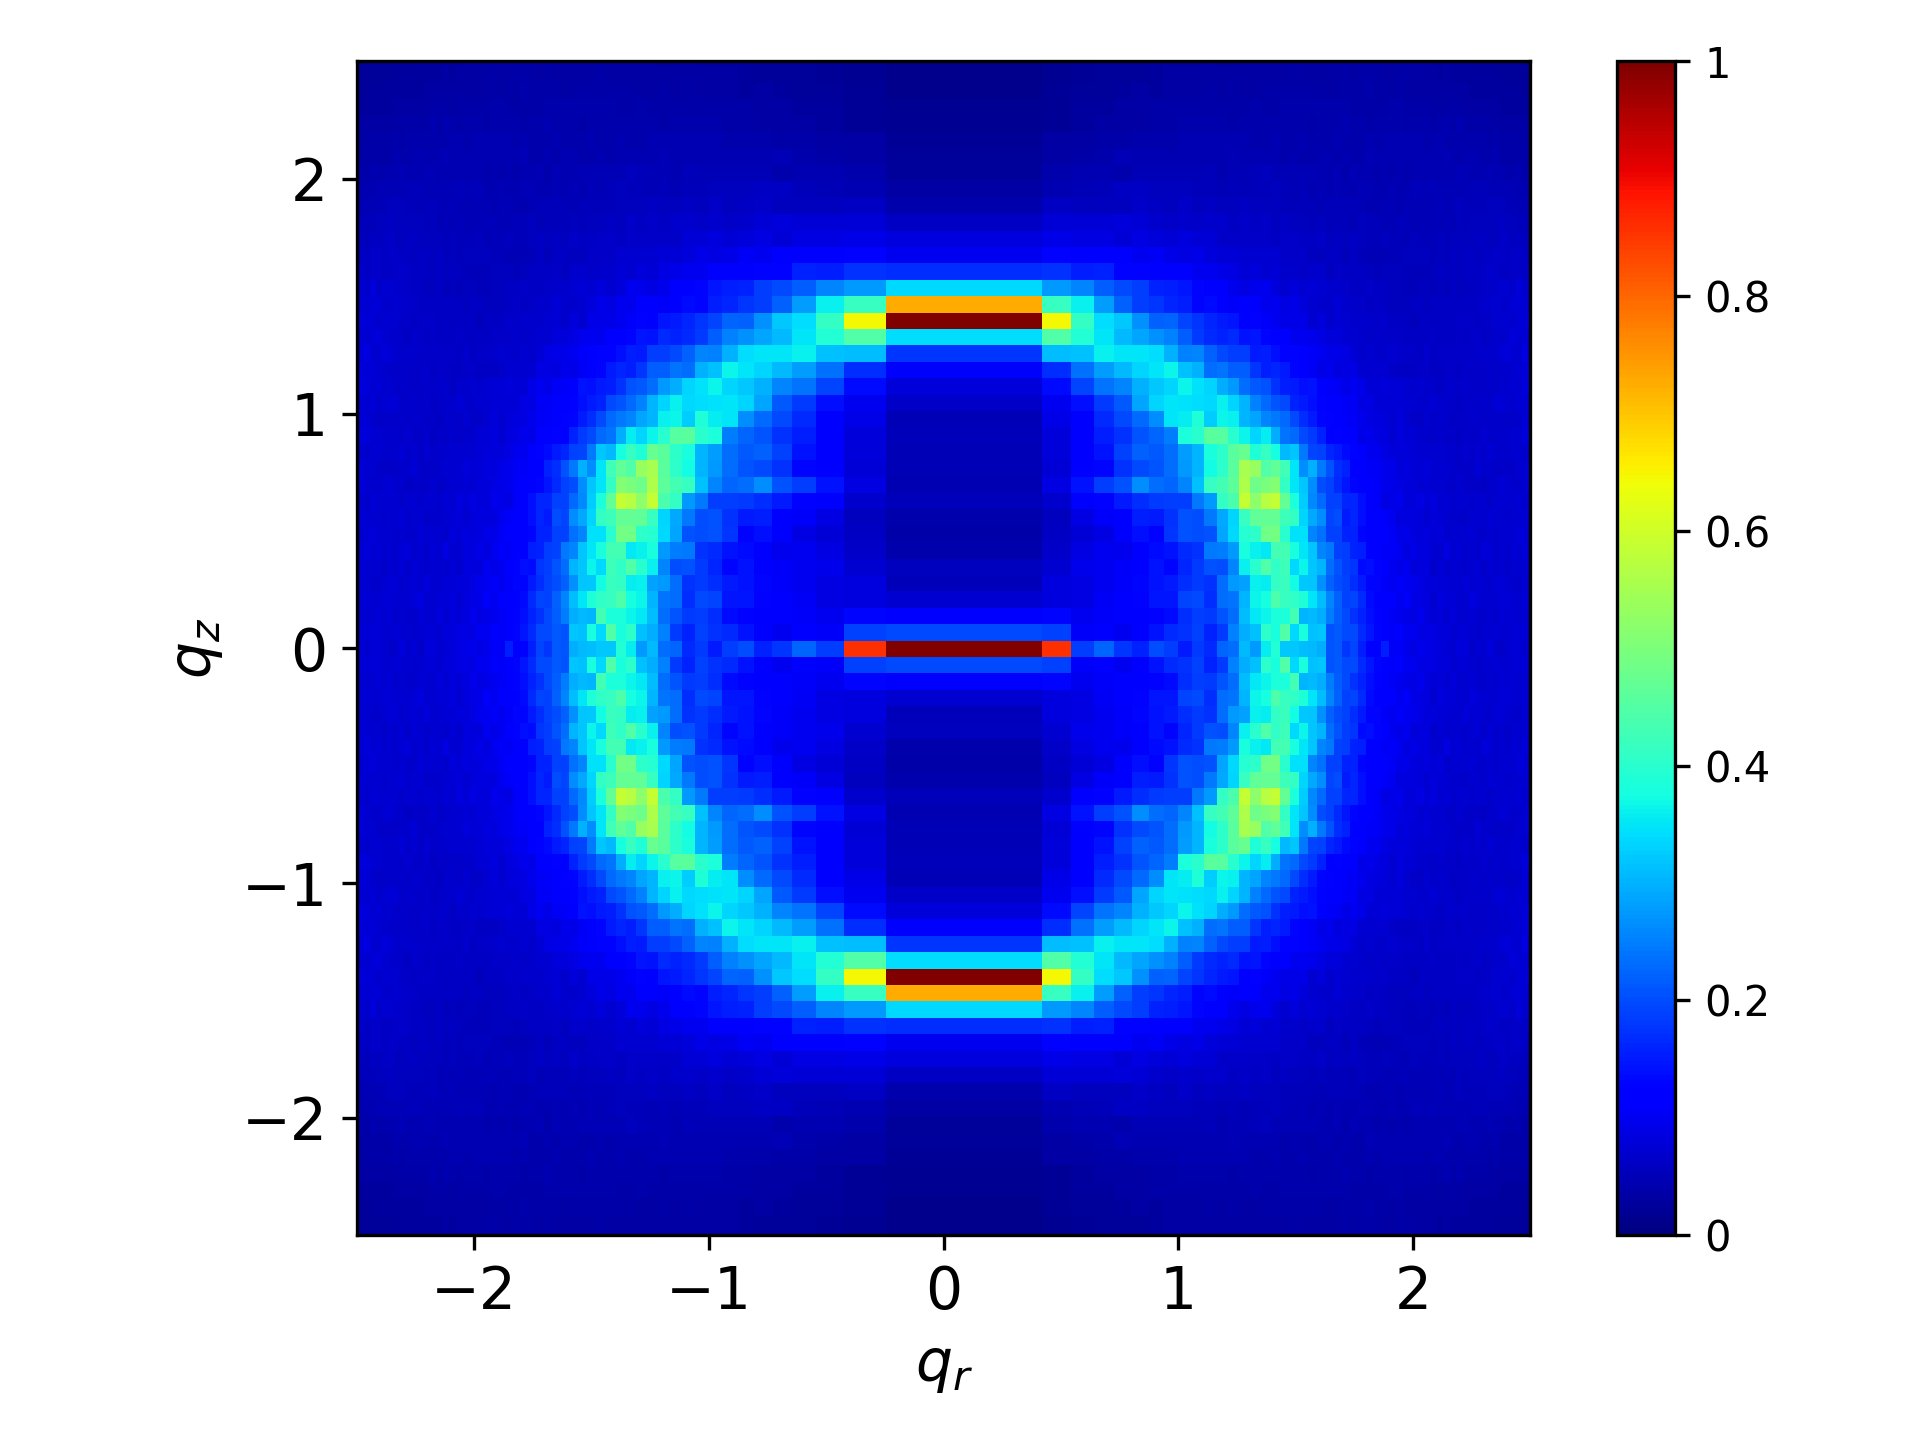
\includegraphics[width=\textwidth]{rzplot_offset_7.png}
                \caption{7 mon/layer, Parallel Displaced}\label{fig:rzplot_offset_7}
        \end{subfigure}
        \begin{subfigure}{0.40\textwidth}
                \centering
                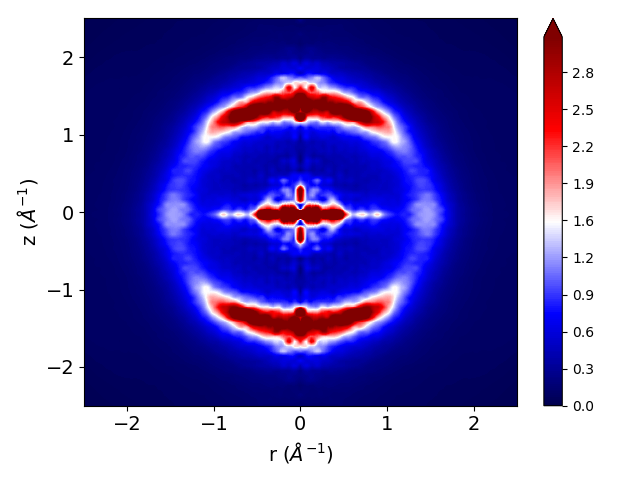
\includegraphics[width=\textwidth]{rzplot_layered_8.png}
                \caption{8 mon/layer, Sandwiched}\label{fig:rzplot_layered_8}
        \end{subfigure}
        \begin{subfigure}{0.40\textwidth}
                \centering
                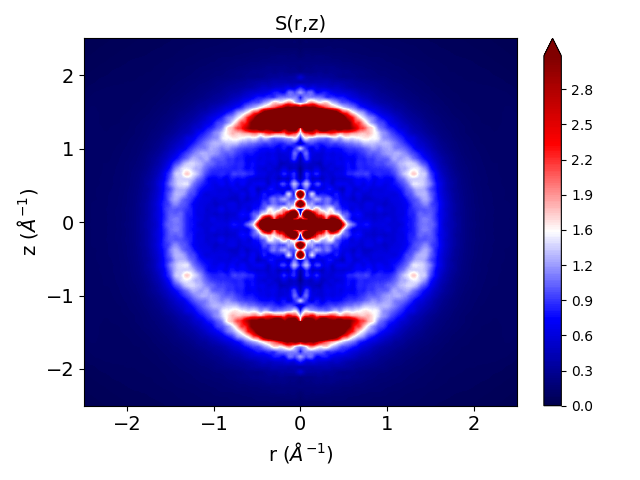
\includegraphics[width=\textwidth]{rzplot_offset_8.png}
                \caption{8 mon/layer, Parallel Displaced}\label{fig:rzplot_offset_8}
        \end{subfigure}
	\caption{Simulated XRD patterns for all other configurations built with
		 layers stacked 3.7 \AA~apart}\label{fig:XRDsim}
  \end{figure}

%  \begin{wrapfigure}{R}{0.4\textwidth}
%      \centering
%      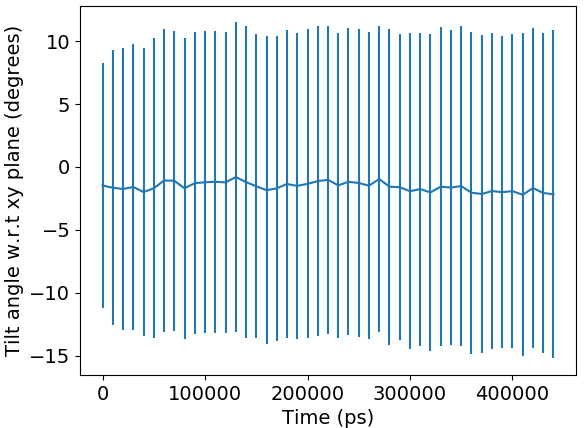
\includegraphics[width=0.4\textwidth]{tilt.png}
%      \caption{The average angle between alkane chains and the xy plane is nearly zero degrees}\label{fig:tilt}     
%  \end{wrapfigure}


%  \begin{figure}
%	\centering
%	\begin{subfigure}{0.45\textwidth}
%		\centering
%		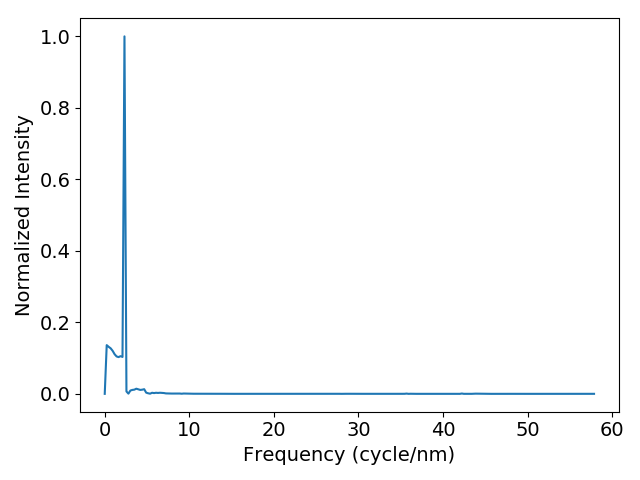
\includegraphics[width=\textwidth]{ps5layered.png}
%		\caption{}\label(fig:ps5layered}
%	\end{subfigure}
%	\begin{subfigure}
%		\centering
%		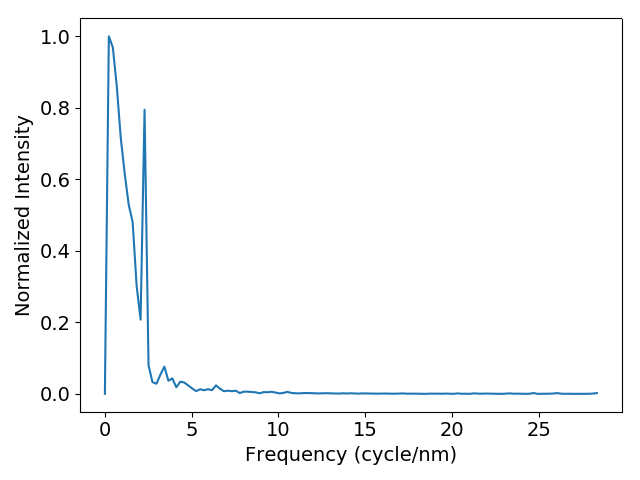
\includegraphics[width=\textwidth]{ps5offset.png}
%		\caption{}\label{fig:ps5offset}
%	\end{subfigure}
%  \end{figure}


  \begin{figure}[!ht]
        \centering
%        \begin{subfigure}{0.45\textwidth}
%                \centering
%                \hspace{-1cm}
%                \vspace{1cm}
%                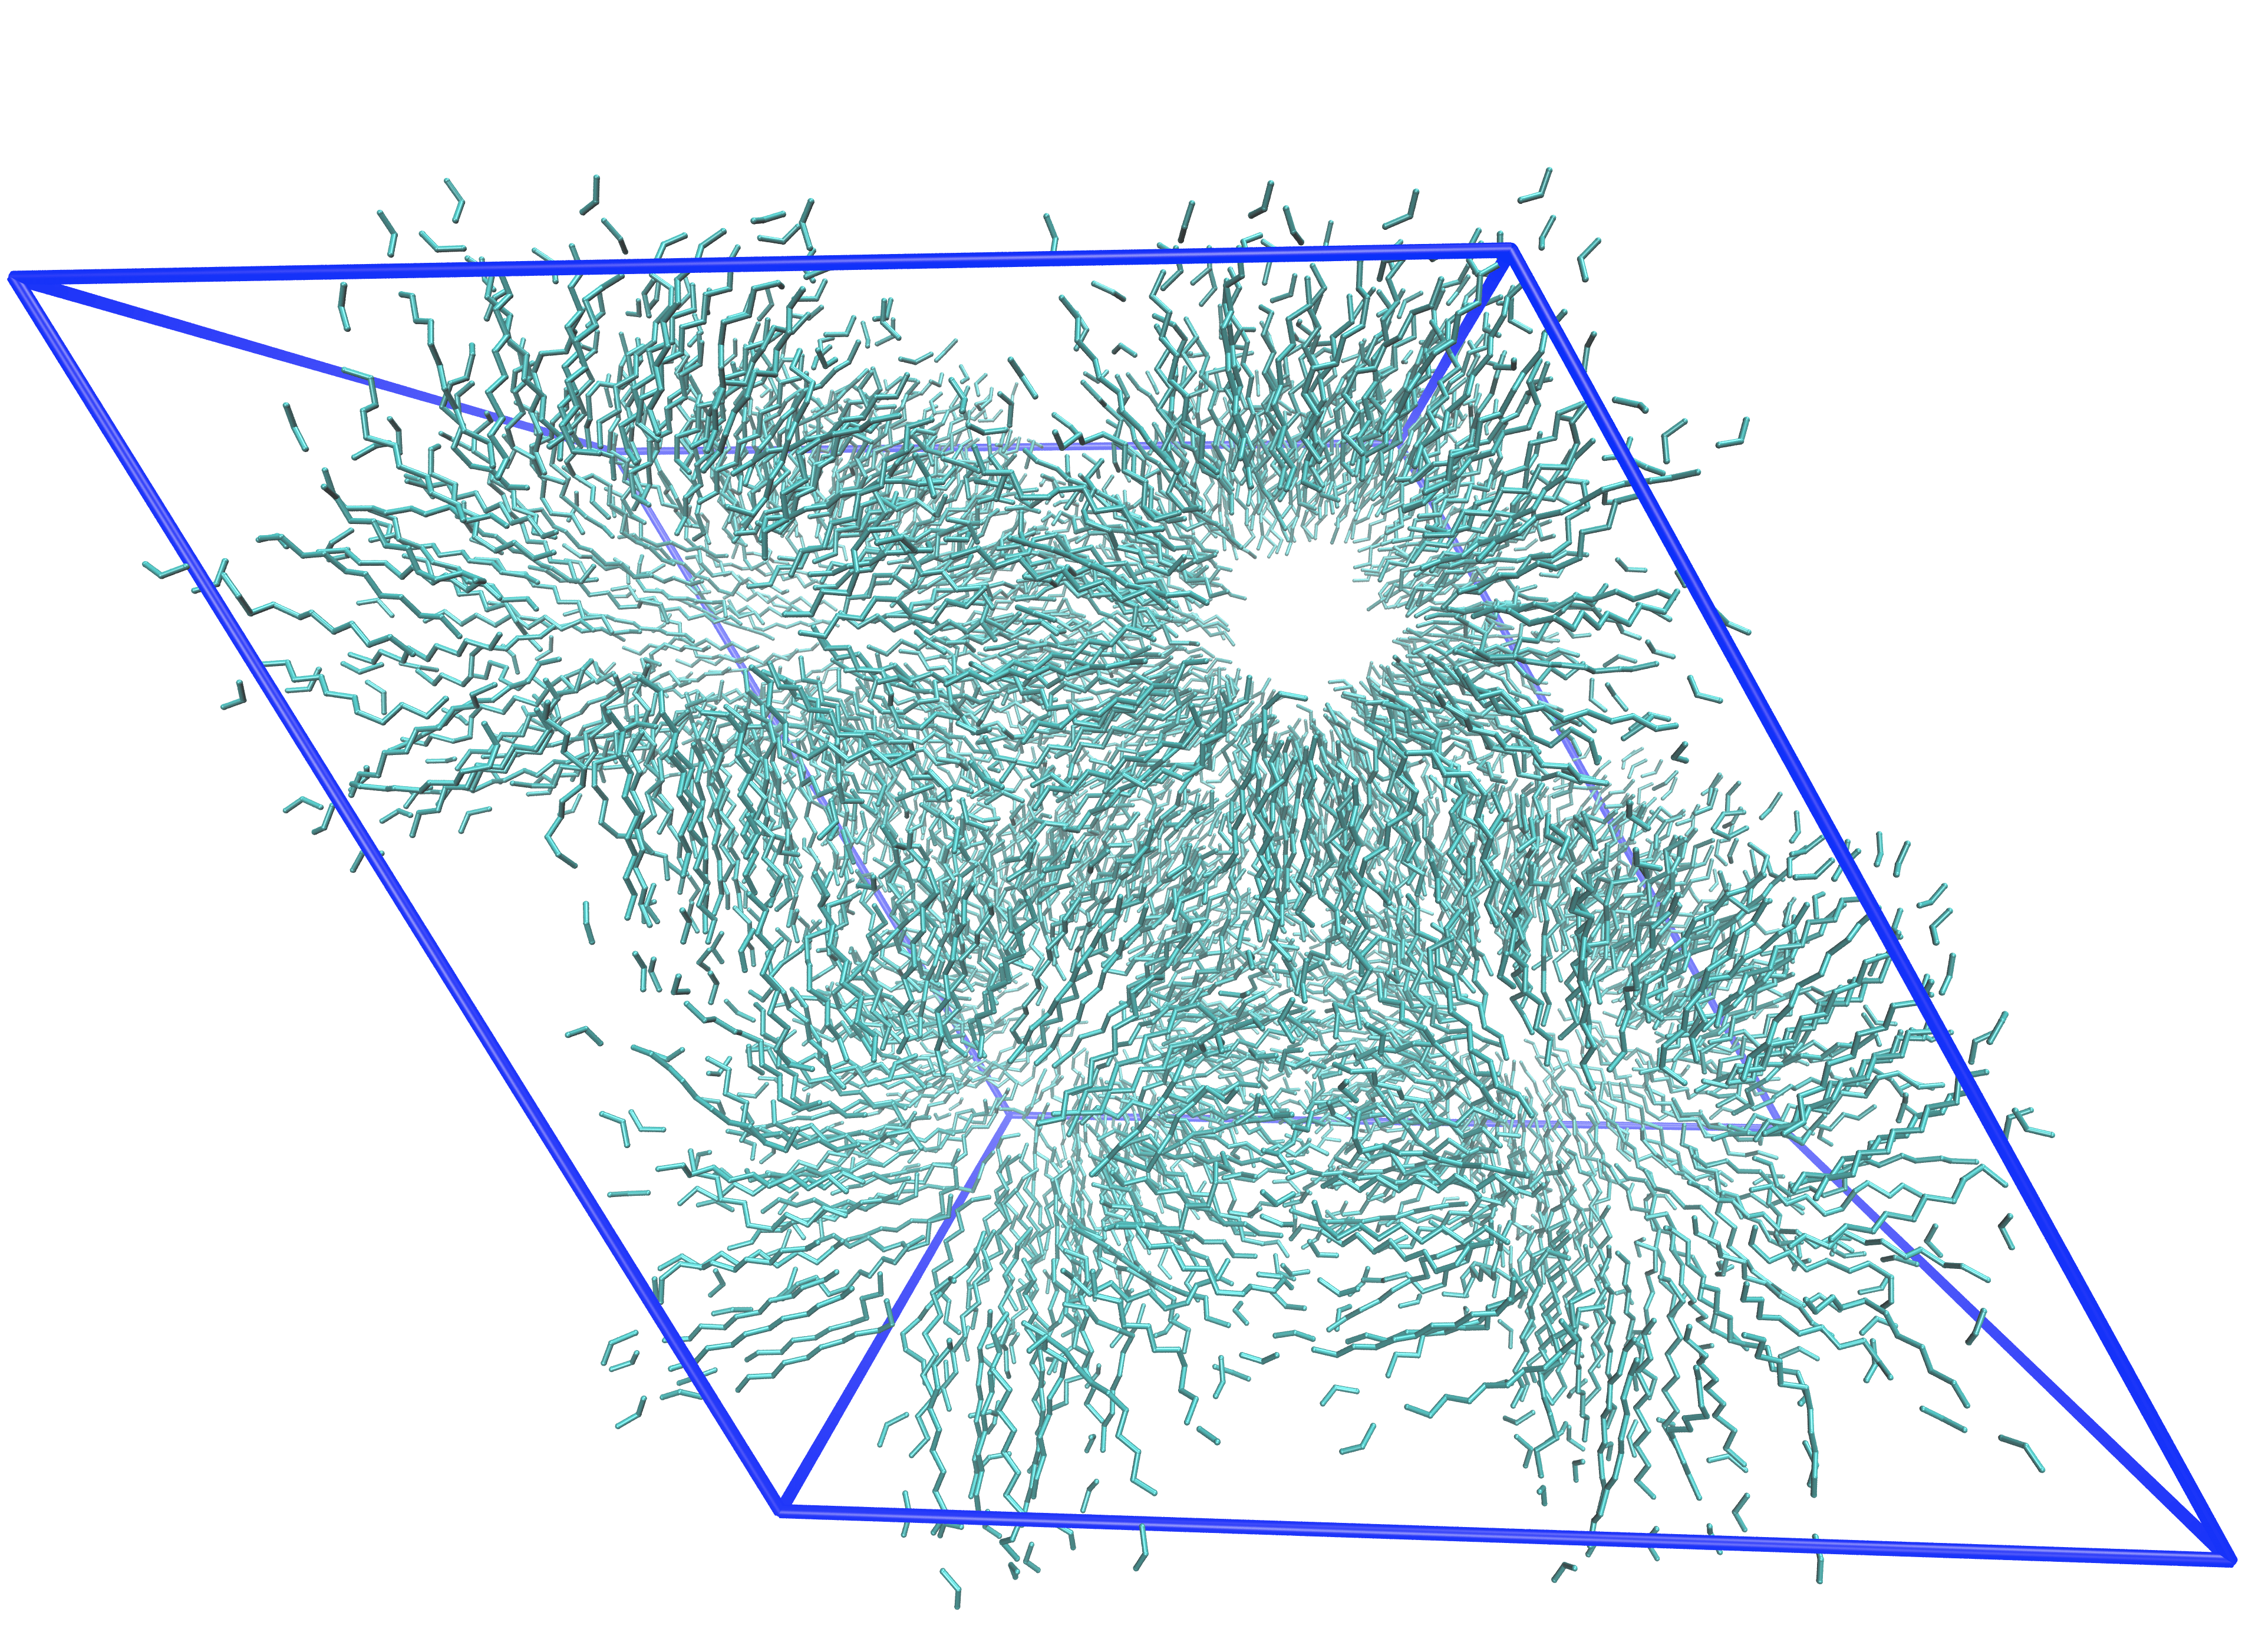
\includegraphics[width=\textwidth,scale=2]{tails_topview.png}
%                \caption{}\label{fig:tails_topview}
%        \end{subfigure}
%        \begin{subfigure}{0.45\textwidth}
%                \centering
%                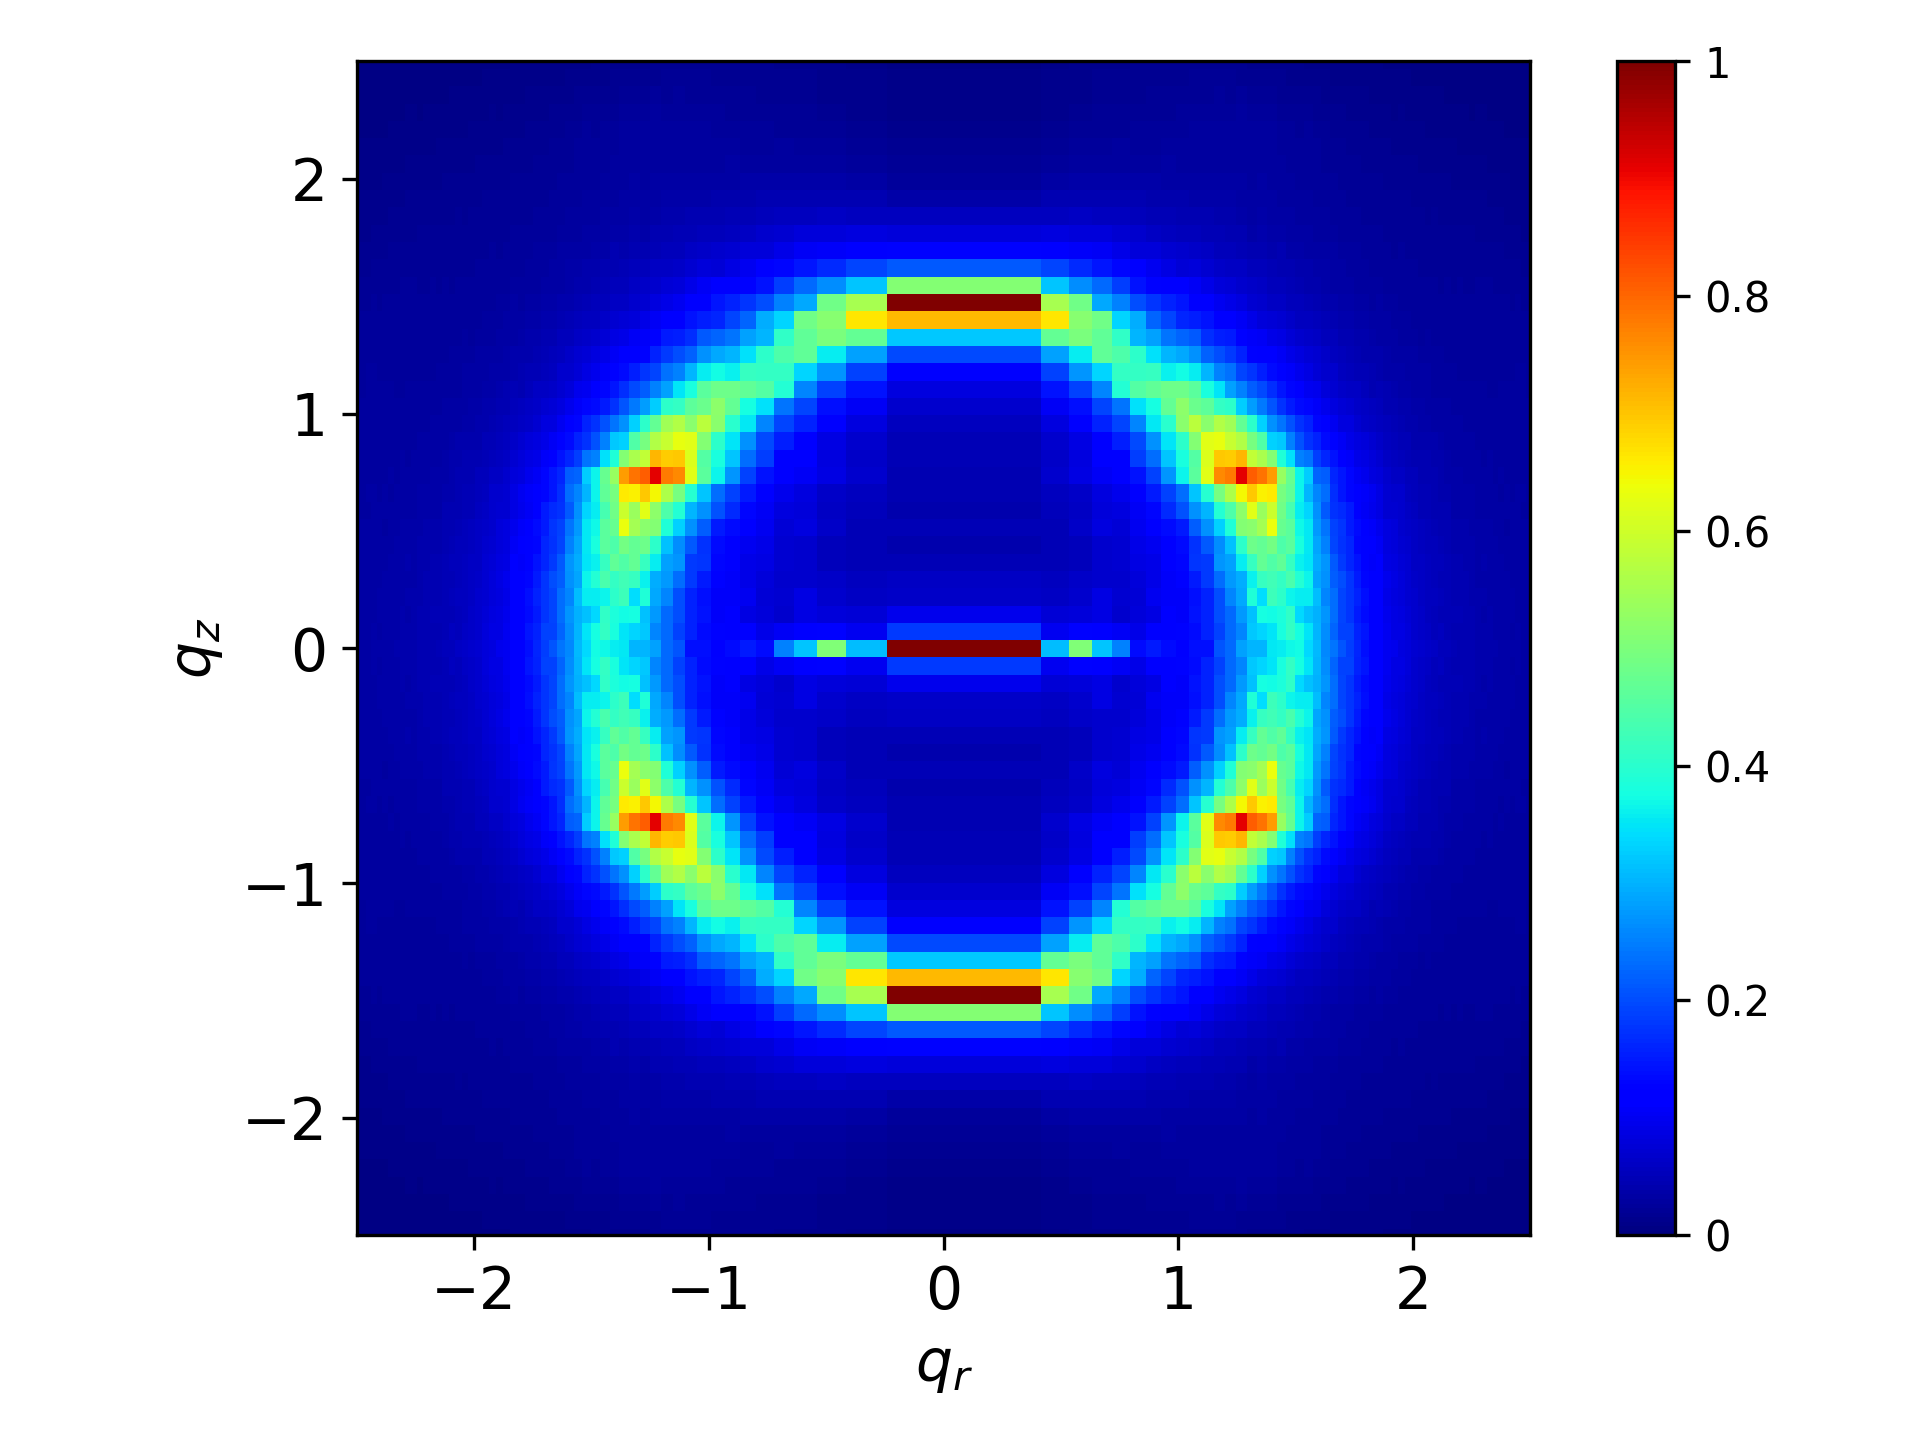
\includegraphics[width=\textwidth]{tails_rzplot.png}
%                \caption{}\label{fig:tails_rzplot}
%        \end{subfigure}
%        \begin{subfigure}{0.45\textwidth}
                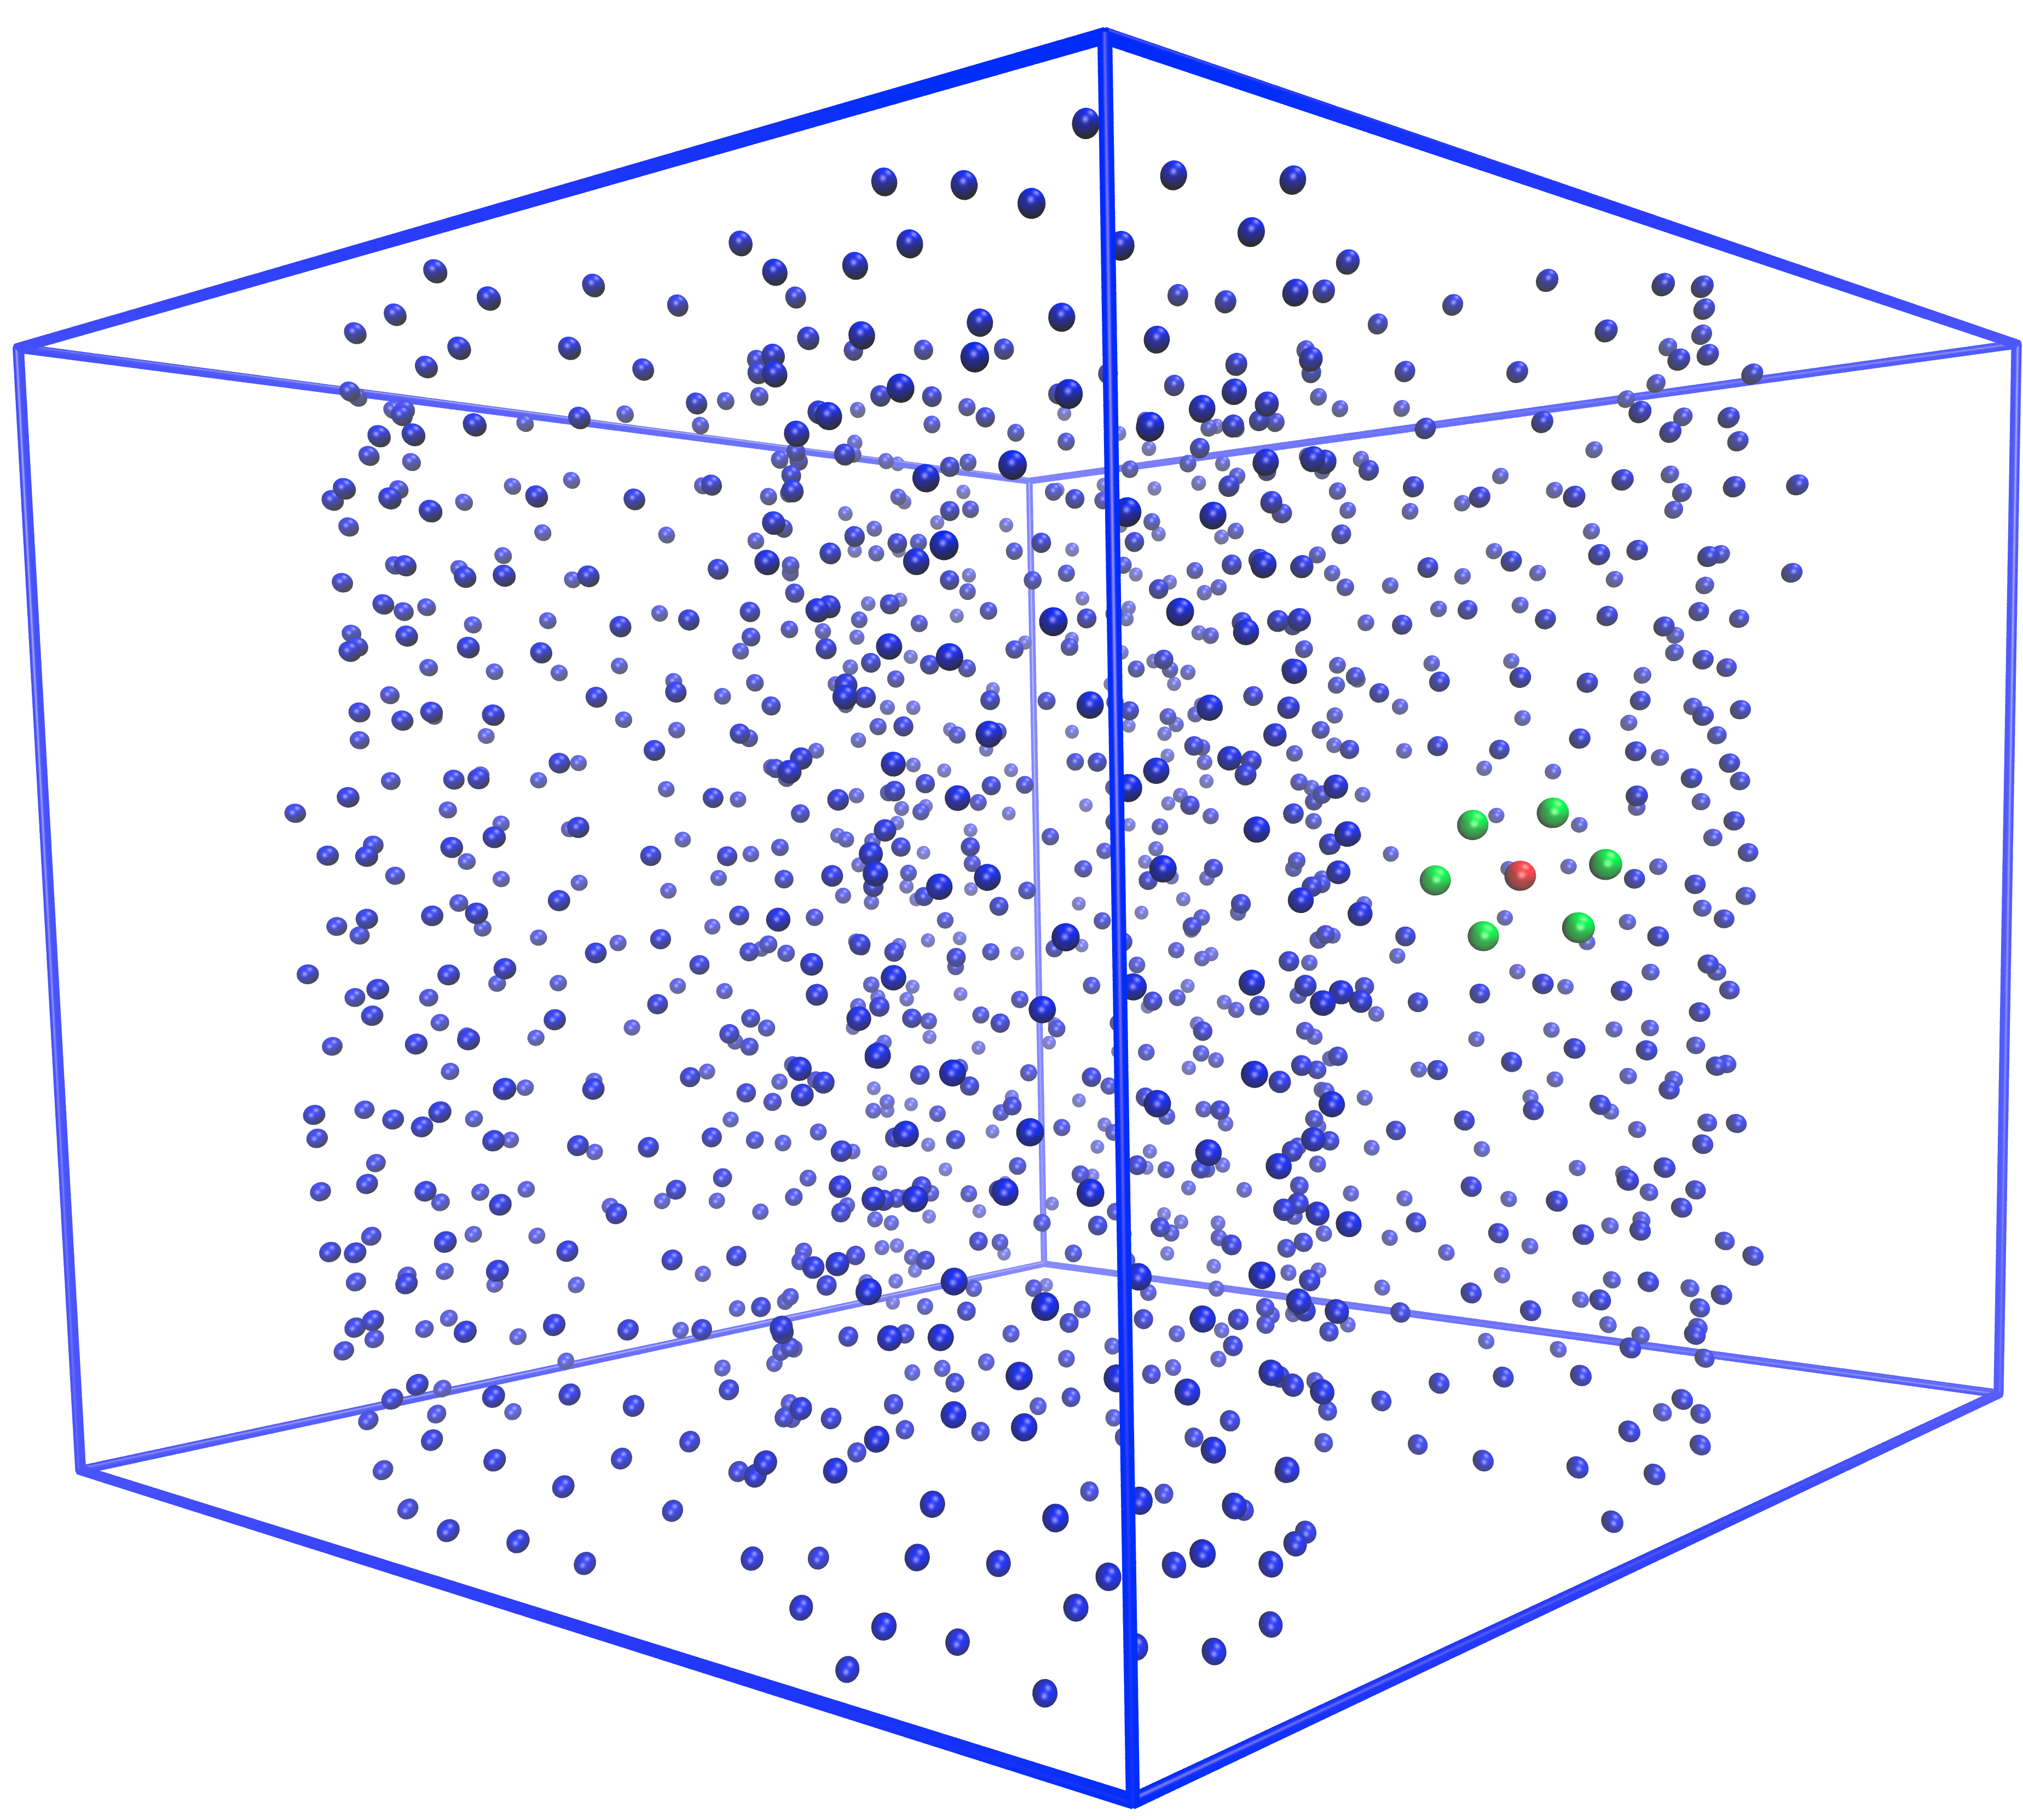
\includegraphics[width=0.5\textwidth]{centroids_box.png}
		\caption{Monomer tails pack together hexagonally. The centroid
			of each tail is visualized as a blue sphere. The centroids are calculated based
			on the red atoms in Figure~\ref{fig:monomer_color_coded}. The red sphere
			highlights an example of an alkane tail centroid with its nearest neighbors
			(green spheres) surrounding it in a hexagonal pattern.}\label{fig:centroids}
%        \end{subfigure}
%        \begin{subfigure}{0.45\textwidth}
%                \centering
%                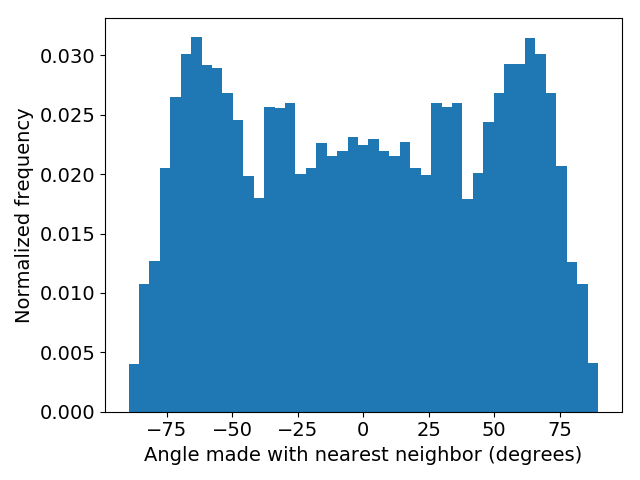
\includegraphics[width=\textwidth]{angles_traj_layered.png}
%                \caption{}\label{fig:angle_distribution}
%        \end{subfigure}
%        \caption{(a) The trajectory can be stripped of all atoms except carbon
%        atoms in monomer tails. (b) Simulated diffraction of the tail-only trajectory
%        still gives rise to R-spots. (c) Finding the center of mass and visualizing
%        their coordinates reveals the hexagonal-like packing of the tails. (d) The
%        distribution created by measuring the angle between each centroid (e.g. red
%        in (c)) and its neareset neighbors (e.g. green in (c)) with respect to the xy
%        plane has distinct spikes near 30\degree, which is consistent with the location
%        of R-spots}\label{fig:tail_packing}
  \end{figure}

  \begin{figure}
  \centering
        \begin{subfigure}{0.45\textwidth}
                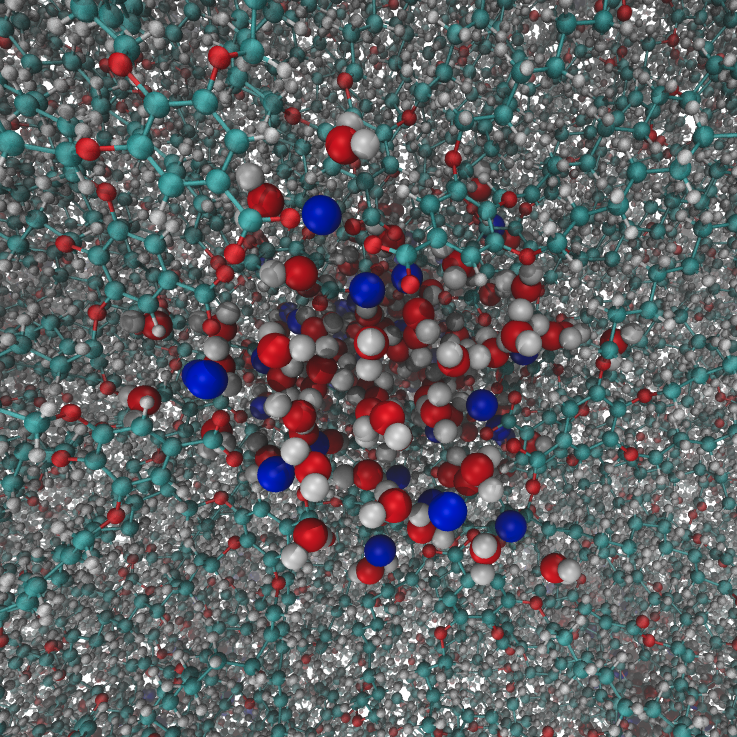
\includegraphics[width=\textwidth]{water_filled_pore.png}
                \caption{}\label{fig:water_filled_pores}
        \end{subfigure}
        \begin{subfigure}{0.45\textwidth}
                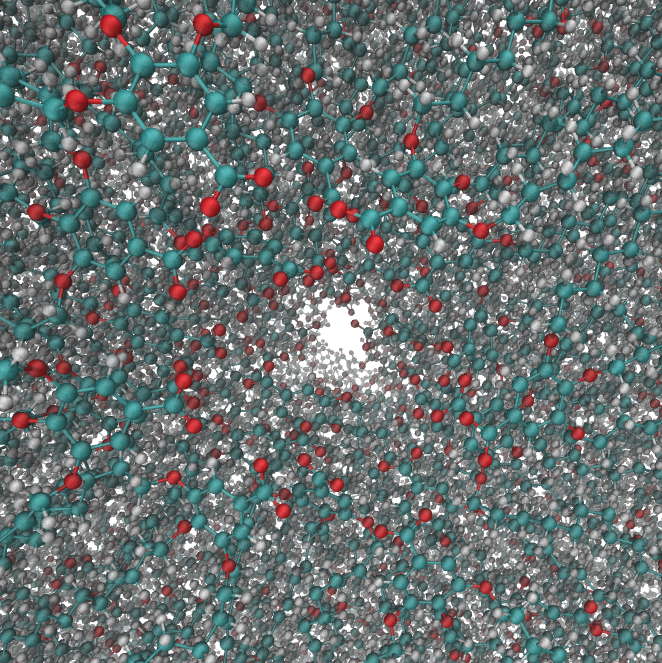
\includegraphics[width=\textwidth]{water_removed.png}
                \caption{}\label{fig:water_removed}
        \end{subfigure}
  \caption{(a) Pores built in the parallel displaced configuration with 5
	  monomers per layer are filled with 5 wt\% water. (b) The same system is
	  visualized with water molecules and sodium ions removed. Head groups vacate the
	  pore region leaving an aqeuous solution of water and sodium ions.}\label{fig:water_pores}
  \end{figure}

\clearpage
\bibliography{llc.bib}
\end{document}
